\PassOptionsToPackage{unicode=true}{hyperref} % options for packages loaded elsewhere
\PassOptionsToPackage{hyphens}{url}
\PassOptionsToPackage{dvipsnames,svgnames*,x11names*}{xcolor}
%
\documentclass[12pt,ngerman,a4paper,ignorenonframetext,]{beamer}
\usepackage{pgfpages}
\setbeamertemplate{caption}[numbered]
\setbeamertemplate{caption label separator}{: }
\setbeamercolor{caption name}{fg=normal text.fg}
\beamertemplatenavigationsymbolsempty
% Prevent slide breaks in the middle of a paragraph:
\widowpenalties 1 10000
\raggedbottom
\setbeamertemplate{part page}{
\centering
\begin{beamercolorbox}[sep=16pt,center]{part title}
  \usebeamerfont{part title}\insertpart\par
\end{beamercolorbox}
}
\setbeamertemplate{section page}{
\centering
\begin{beamercolorbox}[sep=12pt,center]{part title}
  \usebeamerfont{section title}\insertsection\par
\end{beamercolorbox}
}
\setbeamertemplate{subsection page}{
\centering
\begin{beamercolorbox}[sep=8pt,center]{part title}
  \usebeamerfont{subsection title}\insertsubsection\par
\end{beamercolorbox}
}
\AtBeginPart{
  \frame{\partpage}
}
\AtBeginSection{
  \ifbibliography
  \else
    \frame{\sectionpage}
  \fi
}
\AtBeginSubsection{
  \frame{\subsectionpage}
}
\usepackage{lmodern}
\usepackage{amssymb,amsmath}
\usepackage{ifxetex,ifluatex}
\usepackage{fixltx2e} % provides \textsubscript
\ifnum 0\ifxetex 1\fi\ifluatex 1\fi=0 % if pdftex
  \usepackage[T1]{fontenc}
  \usepackage[utf8]{inputenc}
  \usepackage{textcomp} % provides euro and other symbols
\else % if luatex or xelatex
  \usepackage{unicode-math}
  \defaultfontfeatures{Ligatures=TeX,Scale=MatchLowercase}
\fi
\usetheme[]{NPBT}
\usecolortheme{FOM}
\useoutertheme{FOM}
% use upquote if available, for straight quotes in verbatim environments
\IfFileExists{upquote.sty}{\usepackage{upquote}}{}
% use microtype if available
\IfFileExists{microtype.sty}{%
\usepackage[]{microtype}
\UseMicrotypeSet[protrusion]{basicmath} % disable protrusion for tt fonts
}{}
\IfFileExists{parskip.sty}{%
\usepackage{parskip}
}{% else
\setlength{\parindent}{0pt}
\setlength{\parskip}{6pt plus 2pt minus 1pt}
}
\usepackage{xcolor}
\usepackage{hyperref}
\hypersetup{
            pdftitle={Mathematische Grundlagen der Wirtschaftsinformatik},
            pdfauthor={FOM Dozent},
            colorlinks=true,
            linkcolor=blue,
            citecolor=Blue,
            urlcolor=blue,
            breaklinks=true}
\urlstyle{same}  % don't use monospace font for urls
\newif\ifbibliography
\usepackage{color}
\usepackage{fancyvrb}
\newcommand{\VerbBar}{|}
\newcommand{\VERB}{\Verb[commandchars=\\\{\}]}
\DefineVerbatimEnvironment{Highlighting}{Verbatim}{commandchars=\\\{\}}
% Add ',fontsize=\small' for more characters per line
\usepackage{framed}
\definecolor{shadecolor}{RGB}{248,248,248}
\newenvironment{Shaded}{\begin{snugshade}}{\end{snugshade}}
\newcommand{\AlertTok}[1]{\textcolor[rgb]{0.94,0.16,0.16}{#1}}
\newcommand{\AnnotationTok}[1]{\textcolor[rgb]{0.56,0.35,0.01}{\textbf{\textit{#1}}}}
\newcommand{\AttributeTok}[1]{\textcolor[rgb]{0.77,0.63,0.00}{#1}}
\newcommand{\BaseNTok}[1]{\textcolor[rgb]{0.00,0.00,0.81}{#1}}
\newcommand{\BuiltInTok}[1]{#1}
\newcommand{\CharTok}[1]{\textcolor[rgb]{0.31,0.60,0.02}{#1}}
\newcommand{\CommentTok}[1]{\textcolor[rgb]{0.56,0.35,0.01}{\textit{#1}}}
\newcommand{\CommentVarTok}[1]{\textcolor[rgb]{0.56,0.35,0.01}{\textbf{\textit{#1}}}}
\newcommand{\ConstantTok}[1]{\textcolor[rgb]{0.00,0.00,0.00}{#1}}
\newcommand{\ControlFlowTok}[1]{\textcolor[rgb]{0.13,0.29,0.53}{\textbf{#1}}}
\newcommand{\DataTypeTok}[1]{\textcolor[rgb]{0.13,0.29,0.53}{#1}}
\newcommand{\DecValTok}[1]{\textcolor[rgb]{0.00,0.00,0.81}{#1}}
\newcommand{\DocumentationTok}[1]{\textcolor[rgb]{0.56,0.35,0.01}{\textbf{\textit{#1}}}}
\newcommand{\ErrorTok}[1]{\textcolor[rgb]{0.64,0.00,0.00}{\textbf{#1}}}
\newcommand{\ExtensionTok}[1]{#1}
\newcommand{\FloatTok}[1]{\textcolor[rgb]{0.00,0.00,0.81}{#1}}
\newcommand{\FunctionTok}[1]{\textcolor[rgb]{0.00,0.00,0.00}{#1}}
\newcommand{\ImportTok}[1]{#1}
\newcommand{\InformationTok}[1]{\textcolor[rgb]{0.56,0.35,0.01}{\textbf{\textit{#1}}}}
\newcommand{\KeywordTok}[1]{\textcolor[rgb]{0.13,0.29,0.53}{\textbf{#1}}}
\newcommand{\NormalTok}[1]{#1}
\newcommand{\OperatorTok}[1]{\textcolor[rgb]{0.81,0.36,0.00}{\textbf{#1}}}
\newcommand{\OtherTok}[1]{\textcolor[rgb]{0.56,0.35,0.01}{#1}}
\newcommand{\PreprocessorTok}[1]{\textcolor[rgb]{0.56,0.35,0.01}{\textit{#1}}}
\newcommand{\RegionMarkerTok}[1]{#1}
\newcommand{\SpecialCharTok}[1]{\textcolor[rgb]{0.00,0.00,0.00}{#1}}
\newcommand{\SpecialStringTok}[1]{\textcolor[rgb]{0.31,0.60,0.02}{#1}}
\newcommand{\StringTok}[1]{\textcolor[rgb]{0.31,0.60,0.02}{#1}}
\newcommand{\VariableTok}[1]{\textcolor[rgb]{0.00,0.00,0.00}{#1}}
\newcommand{\VerbatimStringTok}[1]{\textcolor[rgb]{0.31,0.60,0.02}{#1}}
\newcommand{\WarningTok}[1]{\textcolor[rgb]{0.56,0.35,0.01}{\textbf{\textit{#1}}}}
\setlength{\emergencystretch}{3em}  % prevent overfull lines
\providecommand{\tightlist}{%
  \setlength{\itemsep}{0pt}\setlength{\parskip}{0pt}}
\setcounter{secnumdepth}{0}

% set default figure placement to htbp
\makeatletter
\def\fps@figure{htbp}
\makeatother

% ===========================================================================
% header.tex
% ==========-----------------------------------------------------------------
%
% (C) in 2017 by Norman Markgraf (nmarkgraf(at)hotmail(dot)com)
%
% ---------------------------------------------------------------------------
%%\AtBeginSection[]{\relax}

\def\logowidth{1.3cm}
\def\logoheight{1.3cm}
\def\logoxshift{-0.85cm}
\def\logoyshift{-0.85cm}

\newcommand\Sinnspruch{\relax}
\newcommand\SinnspruchReset{\renewcommand{\Sinnspruch}{\relax}}
\AtBeginSection[]{%
  %
  % New section, not section in headline
  %
  \setbeamertemplate{headline}[nosectioninhead]
  %
  \begin{frame}
    \frametitle{}
    \vspace*{1.2em}
    {\raggedleft\textit{\Sinnspruch}}
    \vspace*{7cm}
    \begin{tikzpicture}[remember picture, overlay]
      \putLogo%
      \node[% section title
          xshift=\logoxshift-6.6cm,
          %anchor=south east,
          yshift=3.8cm, 
          inner sep=0pt
      ] at (current page.south east){%
%          \fbox{
            \makebox[\sectiontitleboxwidth][r]{%
              {%
                \usebeamercolor{sectionnumber title}%
                \usebeamerfont{sectionnumber title}\insertsectionnumber\hspace*{0.15em}%
              }%
              {%
                \usebeamercolor[fg]{section title}%
                \usebeamerfont{section title}\NoHyper\insertsectionhead\endNoHyper%
              }
            }% makebox
%          }% fbox
    };% war mal -3pt
     \node[% 
        anchor=west, 
        inner sep=0pt, % 13pt 
        xshift=13pt,
        yshift=-\logoheight-12pt
      ] at (current page.north west){
            \logoline
          };
    \end{tikzpicture}%
  \end{frame}
  % Reset headline. Put section in head
  \setbeamertemplate{headline}[sectioninhead]
%  \addtocounter{framenumber}{-1}% If you don't want them to affect the slide number
}

\AtBeginSubsection[]{%
  %
  % New subsection, not section in headline
  %
  \setbeamertemplate{headline}[nosectioninhead]
  %
  \begin{frame}
    \frametitle{}
    \vspace*{1.2em}
    {\raggedleft\textit{\Sinnspruch}}
    \vspace*{7cm}
    \begin{tikzpicture}[remember picture, overlay]
%    \node[inner sep=0pt] at (current page.center){%
%              \includegraphics[width=\myPaperWidth,height=\myPaperHeight]{\backgroundimage}%
%      };%
      \node[% Logo
        shift={(\logoxshift,\logoyshift)},
        inner sep=0pt] at (current page.north east){%
              \includegraphics[%
                  width=\logowidth,
                  height=\logoheight
              ]{\logoimage}%
      };% ,xshift=-1cm,yshift=4cm
      \node[% section title
          xshift=\logoxshift-6.6cm,
          %anchor=south east,
          yshift=3.8cm, 
          inner sep=0pt
      ] at (current page.south east){%
%          \fbox{
            \makebox[\sectiontitleboxwidth][r]{%
              {%
                \usebeamercolor{sectionnumber title}%
                \usebeamerfont{sectionnumber title}\insertsectionnumber.%\insertsubsectionnumber\hspace*{0.15em}%
              }%
              {%
                \usebeamercolor{subsectionnumber title}%
                \usebeamerfont{subsectionnumber title}\insertsubsectionnumber\hspace*{0.15em}%
              }%
              {%
                \usebeamercolor[fg]{subsection title}%
                \usebeamerfont{subsection title}\NoHyper\insertsubsectionhead\endNoHyper%
              }
            }% makebox
%          }% fbox
    };% war mal -3pt
     \node[% 
        anchor=west, 
        inner sep=0pt, % 13pt 
        xshift=13pt,
        yshift=-\logoheight-12pt
      ] at (current page.north west){
            \logoline
          };
    \end{tikzpicture}%
  \end{frame}
  % Reset headline. Put section in head
  \setbeamertemplate{headline}[sectioninhead]
%  \addtocounter{framenumber}{-1}% If you don't want them to affect the slide number
}



\setbeamertemplate{section in toc}{%
    \leavevmode\leftskip=2.75ex%
  \llap{%
    \usebeamerfont*{section number projected}%
    \usebeamercolor[bg]{section number projected}%
    \vrule width2.50ex height2.05ex depth.4ex%
    \hskip-2.50ex%
    \hbox to2.50ex{\hfil\color{fg}\inserttocsectionnumber\hfil}}%
  \kern1.35ex\inserttocsection\par}

%
% BUGFIX für caption bug in 2018!
% 
% see: https://tex.stackexchange.com/questions/426088/texlive-pretest-2018-beamer-and-subfig-collide/426090#426090
% see: https://www.mrunix.de/forums/showthread.php?77329-Undefined-control-sequence-magyar-captionfix-beim-Laden-von-subfig-in-beamer
% see: https://gitlab.com/axelsommerfeldt/caption/issues?state=opened
%
\makeatletter
\let\@@magyar@captionfix\relax
\makeatother

\InputIfFileExists{include-notes.tex}{\relax}{\relax}
\InputIfFileExists{header_costums.tex}{\relax}{\relax}
% ===========================================================================
\ifnum 0\ifxetex 1\fi\ifluatex 1\fi=0 % if pdftex
  \usepackage[shorthands=off,main=ngerman]{babel}
\else
  % load polyglossia as late as possible as it *could* call bidi if RTL lang (e.g. Hebrew or Arabic)
  \usepackage{polyglossia}
  \setmainlanguage[]{german}
\fi

\title{Mathematische Grundlagen der Wirtschaftsinformatik}
\author{FOM Dozent}
\providecommand{\institute}[1]{}
\institute{FOM}
\date{}

\begin{document}
\frame{\titlepage}

% ===========================================================================
% before.tex
% ==========-----------------------------------------------------------------

%
% New section, not section in headline
%
\mode<beamer>
  \setbeamertemplate{headline}[nosectioninhead]
\mode<all>
\begin{frame}
  \frametitle{Inhaltsverzeichnis}
  %\vspace*{-1cm}%
  \flushcolumns % \raggedcolumns% 
  \setlength{\columnsep}{0.2cm}%
  \begin{multicols}{2}
    \tableofcontents[hideallsubsections]
  \end{multicols}
\end{frame}
\mode<beamer>
  \setbeamertemplate{headline}[sectioninhead]
\mode<all>
% Läuft nicht ... leider ...
%\makeatletter
%  \beamer@tocsectionnumber=-1\relax
%  setcounter{section}{-1}
%\makeatother

%
% Eigentlich sollte das Kapitel "0" nicht dargestellt werden. 
% Also "Organisatorische" sollte nicht wirklich eine Nummer tragen 
% oder wenn, dann die Nummer 0. --- FIX ME ---
%
%\mode<beamer>
%\addtocounter{section}{-1}
%\mode<*>
% ===========================================================================

\hypertarget{organisatorisches}{%
\section{Organisatorisches}\label{organisatorisches}}

\begin{frame}{Literatur (Auswahl)}
\protect\hypertarget{literatur-auswahl}{}

\begin{itemize}
\tightlist
\item
  Christiaans,Thomas; Ross, Matthias: \emph{Wirtschaftsmathematik für
  das Bachelor-Studium}, Springer Gabler, 2013
  \url{https://www.openintro.org/stat/textbook.php?stat_book=isrs}
\item
  Hartmann, Peter: \emph{Mathematik für Informatiker Taschenbuch}, 6.
  Auflage, Springer Vieweg, 2015, ISBN: 978-3658034153
\item
  Luderer, Bernd; Würker, Uwe: \emph{Einstieg in die
  Wirtschaftsmathematik}, 9. Auflage, Springer Gabler Verlag, 2015
\end{itemize}

\end{frame}

\begin{frame}[fragile]{Lizenz\thinspace{}/\thinspace{}Version}
\protect\hypertarget{lizenz-version}{}

Diese Folien wurden von Norman Markgraf zusammen mit Kolleg*innen von
der FOM \url{https://www.fom.de/} entwickelt und stehen unter der Lizenz
CC-BY-SA-NC 3.0 de:
\url{https://creativecommons.org/licenses/by-nc-sa/3.0/de/}

Der verwendete Code sowie das Beamer Template aus dem
\href{http://github.com/NMarkgraf/NPBT}{NPBT-Projekt} von Norman
Markgraf stehen unter der Lizenz
\href{https://www.gnu.org/licenses/gpl-3.0.de.html}{GNU General Public
License v3.0}.

\begin{itemize}
\tightlist
\item
  Datum erstellt: 2018-09-17
\item
  R Version: 3.5.1
\item
  \texttt{mosaic} Version: 1.4.0
\end{itemize}

Bitte melden Sie Fehler und Verbesserungsvorschläge:
\href{mailto:nmarkgraf@hotmail.de}{\nolinkurl{nmarkgraf@hotmail.de}}

Mitarbeit und Hinweise von Thomas Christiaans, Mathias Ross, Oliver
Gansser, Matthias Gehrke, Jörg Horst, Bianca Krol, Karsten Lübke,
Sebastian Sauer, Daniel Ziggel. \textbf{Vielen Dank!}

\end{frame}

\begin{frame}{Lernergebnisse}
\protect\hypertarget{lernergebnisse}{}

Die Studierenden können nach erfolgreichem Abschluss des Moduls:

\begin{itemize}
\tightlist
\item
  die grundlegenden Methoden der diskreten Mathematik, der Algebra und
  der Analysis anwenden und auf weitere wirtschaftsinformatische und
  informationstechnische Anwendungen (zum Beispiel Softwareentwicklung,
  Datenbankmanagement und Netzwerktechnik) übertragen,
\item
  Aufgaben /\thinspace{}Übungen des Themengebiets berechnen und lösen,
\item
  arithmetische und analytische Methodiken auswählen,
\item
  die fachlichen Begrifflichkeiten verstehen und anwenden,
\item
  Beweismethoden nachvollziehen,
\item
  die Anwendbarkeit mathematischer Methoden im Unternehmen beurteilen.
\end{itemize}

\end{frame}

\begin{frame}{Prüfungsleistung}
\protect\hypertarget{prufungsleistung}{}

\begin{itemize}
\tightlist
\item
  100 \% \textbf{Klausur} 90 Minuten. Zur Vergabe von Credit Points muss
  die Klausur mit einer mindestens ausreichenden Leistung bestanden
  werden.
\end{itemize}

\textbf{Beachten Sie die im OC hinterlegten Fristen!}

Workload:

\begin{itemize}
\tightlist
\item
  Präsenzstunden: 40,0 UE
\item
  Strukturiertes Eigenstudium 95,00 ZStd
\item
  Workload gesamt: 125,0 ZStd
\item
  ECTS-Credit Punkte: 5
\end{itemize}

\end{frame}

\begin{frame}{Bitte}
\protect\hypertarget{bitte}{}

\begin{itemize}
\tightlist
\item
  Stellen Sie ein Namensschild auf.
\item
  Seien Sie offen für das Thema.
\item
  Haben Sie Respekt aber keine Angst vor der Schwierigkeit des Themas.
\item
  Bereiten Sie den Lehrstoff von Anfang an kontinuierlich nach.
\item
  Stellen Sie Fragen!
\item
  Sie können Sich gerne während der Übungen unterhalten, aber nicht wenn
  ich etwas erkläre -- das ist u.\thinspace{}a. auch unfair!
\item
  Versuchen Sie die Übungen selbst zu lösen - der Lernerfolg ist
  ungleich größer, als wenn Sie die Lösung ``abnicken''. Für die Quizze
  wird ein Live-Feedback-System eingesetzt: \url{https://tweedback.de/}
  \textbf{Nehmen Sie daran teil!}\footnote<.->{Siehe
    \mbox{z.\thinspace{}B.}\xspace{}
    \href{https://doi.org/10.1177/0098628314562685}{Nguyen, K., \&
    McDaniel, M.\thinspace{}A. (2015). Using quizzing to assist student
    learning in the classroom: the good, the bad, and the ugly. Teaching
    of Psychology, 42(1), 87-92}.}
\item
  Versuchen Sie Ablenkungen (Facebook, WhatsApp etc.) zu
  vermeiden.\footnote<.->{Siehe \mbox{z.\thinspace{}B.}\xspace{}
    \href{https://doi.org/10.1016/j.compedu.2012.10.003}{Sana, F.,
    Weston, T., \& Cepeda, N.\thinspace{}J. (2013). Laptop multitasking
    hinders classroom learning for both users and nearby peers.
    Computers \& Education, 62, 24-31}.} .
\end{itemize}

\end{frame}

\begin{frame}{Hinweis}
\protect\hypertarget{hinweis}{}

\textbf{Bleiben Sie dran!}

\textbf{Die Inhalte bauen aufeinander auf},
\mbox{d.\thinspace{}h.,}\xspace{} arbeiten Sie nach. Die angegebene
Literatur ist frei verfügbar. Wenn Sie nicht \textbf{kontinuierlich
nacharbeiten} wird es immer schwerer, da immer mehr Grundlagen fehlen.

Ich kann versuchen, es Ihnen zu erklären, ich kann es \emph{nicht} für
Sie verstehen. Daher: fragen Sie direkt in der nächsten Vorlesung nach,
wenn Sie in der Nacharbeit etwas nicht verstanden haben.

Die Folien bilden die \emph{Leinwand} der Vorlesung: sie werden
\emph{interaktiv} erklärt und ergänzt.

\end{frame}

\begin{frame}{Keine Tipps}
\protect\hypertarget{keine-tipps}{}

Tipps von (fiktiven) Studierenden:

\begin{itemize}
\tightlist
\item
  Ich besuche die Vorlesung nicht, ich gucke Videos.
\item
  Kontinuierlich nacharbeiten? Quatsch, ich lerne eine Woche vor der
  Klausur intensiv.
\item
  Es reicht, wenn ich mit einem halben Ohr zuhöre -- ich spiele, chatte,
  surfe während der Vorlesung.\footnote<.->{vgl.
    \url{https://youtu.be/vJG698U2Mvo}}
\item
  Mitschreiben? Ich mache, wenn überhaupt, ein Foto.\footnote<.->{Hier
    \textbf{nicht} erlaubt.}
\item
  Selbstlernunterlagen und Literatur habe ich nicht nötig.
\item
  Mir genügt die Übungsklausur zur Klausurvorbereitung -- falls eine
  angeboten wird.
\item
  Übungen selber lösen? -- Es reicht, wenn ich die Lösung kenne.
\end{itemize}

Manche dieser Studierenden haben es leider \textbf{nicht} geschafft.

\textbf{Sie} können es \textbf{besser}!\footnote<.->{Siehe
  \mbox{z.\thinspace{}B.}\xspace{} echte Tipps unter
  \href{https://doi.org/10.1177/1745691616645770}{Putnam,
  A.\thinspace{}L., Sungkhasettee, V.\thinspace{}W., \& Roediger III,
  H.\thinspace{}L. (2016). Optimizing learning in college: tips from
  cognitive psychology. Perspectives on Psychological Science, 11(5),
  652-660.}}

\end{frame}

\hypertarget{mengen}{%
\section{Mengen}\label{mengen}}

\begin{frame}{Über den Begriff der Menge}
\protect\hypertarget{uber-den-begriff-der-menge}{}


\begin{columns}[T]
	\begin{column}[t]{0.74\textwidth}

Was dachte der Vater der Mengenlehre einst, was Mengen sind:

\begin{center}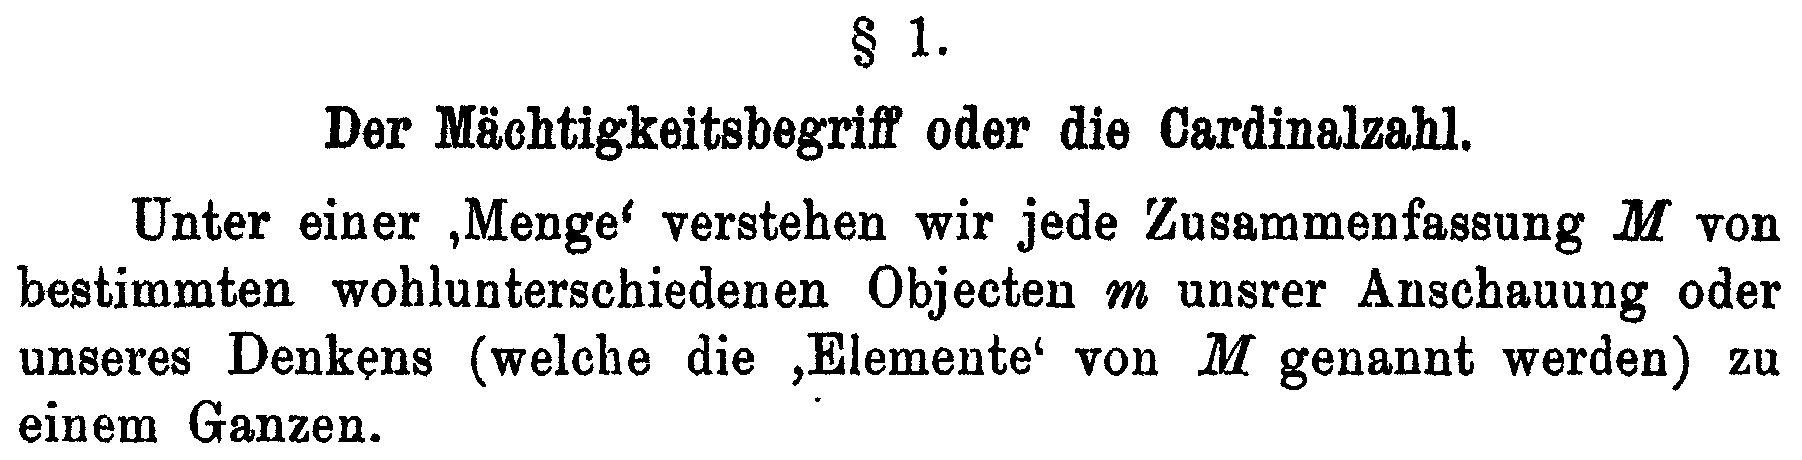
\includegraphics[width=0.95\linewidth]{./images/MGWI/TextstelleMitDerMengendefinitionVonGeorgCantor} \end{center}

{\tiny{}

Quelle: \href{http://bit.ly/1QSwuoV}{Beiträge zur Begründung der
transfiniten Mengenlehre} -- Mathematische Annalen (Zeits.-band 46) -
1915

}


	\end{column}
	\begin{column}[t]{0.24\textwidth}
\personDB{Cantor}
	\end{column}
\end{columns}


\begin{Bemerkungen}[]

{\scriptsize{}

Felix Bernstein, ein Schüler von Cantor, berichtete von Richard Dedekind
Folgendes:

Dedekind habe gesagt, für ihn seien Mengen \glqq geschlossene Säcke, die
ganz bestimmte Dinge enthalten, von denen man nichts wisse, außer, dass
sie vorhanden und bestimmt seien\grqq.

Cantor habe daraufhin \glqq seine kolossale Figur\grqq\textasciitilde{}
aufgerichtet, erinnerte sich Bernstein: \glqq Er beschrieb mit erhobenem
Arm eine großartige Geste und sagte mit einem ins Unbestimmte
gerichteten Blick: \glq Eine Menge stelle ich mir vor wie einen
Abgrund.\grq \grqq

{{\tiny{}Quelle: \href{http://bit.ly/1KFCxwf}{Die Zahlengerade kennt
jeder aus der Schulzeit}}}

}

\end{Bemerkungen}

\end{frame}

\begin{frame}{Darstellungsformen von Mengen}
\protect\hypertarget{darstellungsformen-von-mengen}{}

\begin{itemize}
\item
  \textbf{Explizite /\thinspace{}Aufzählende Darstellung}

  Man kann die Elemente der Menge \emph{aufzählen}: \begin{equation*}
        \{ 3, 4, 5, 6 \}
    \end{equation*}
\item
  \textbf{Implizite /\thinspace{}Beschreibende Darstellung}

  Man beschreibt \emph{Eigenschaften}/\emph{Merkmale} der Elemente die
  zur Menge gehören.\\
  Für ``die \tikz[baseline]{
                        \node[fill=blue!20,anchor=base,rounded corners] (t1)
                            {Menge aller natürlichen Zahlen $x$};
                    }, \tikz[baseline]{
                        \node[fill=red!20,anchor=base,rounded corners] (t2)
                            {für die gilt};
                    }: \tikz[baseline]{
                        \node[fill=green!20,anchor=base,rounded corners] (t3)
                            {x ist größer als 2 und kleiner als 7};
                    }.''\xspace schreibt man auch kurz:
  \begin{equation*}
                        \{
                            \tikz[baseline=-.5ex]{\node[fill=blue!20,rounded corners]  (n1) {$x \in \mathbf{N}$};}
                            \tikz[baseline=-.5ex]{\node[fill=red!20,rounded corners]   (n2) {$\,|\,$};}
                            \tikz[baseline=-.5ex]{\node[fill=green!20,rounded corners] (n3) {$2 < x < 7$};} 
                        \}
    \end{equation*}
\item
  \textbf{Venn- /\thinspace{}Mengen-Diagramme}

  \begin{center}
    \begin{tikzpicture}
        \begin{scope}
            \draw (0,0) ellipse (25pt and 18pt);                
        \end{scope}
        \node at (-0.5, 0  ) {$3$};
        \node at (   0, 0.1) {$5$};
        \node at ( 0.5, 0.3) {$4$};
        \node at (-0.3,-0.3) {$6$};
    \end{tikzpicture}
    \end{center}
\end{itemize}

\end{frame}

\begin{frame}{Übung 1:}
\protect\hypertarget{ubung-1}{}

Geben Sie die folgende Mengen in der aufzählenden Darstellungsform an:

\begin{enumerate}
[a)]
\tightlist
\item
  \(\displaystyle A_1 = \left\{x \in \mathbf{N} \,|\, x \neq 6 \text{ und } x \text{ gerade und } x < 10 \right\}\)
\item
  \(\displaystyle A_2 = \left\{x \in \mathbf{N} \,|\, x = 2 \cdot n \text{ mit } n \in \mathbf{N} \text{ und } x < 10 \right\}\)
\end{enumerate}

Geben Sie die folgende Mengen in der impliziter Darstellungsform an:

\begin{enumerate}
[a)]
\setcounter{enumi}{2}
\tightlist
\item
  \(\displaystyle A_3 = \left\{7, 21, 14, 28, 35 \right\}\)
\item
  \(\displaystyle A_4 = \left\{10,8,2,4,2,8,6,10 \right\}\)
\end{enumerate}

\note{\begin{enumerate}
[a)]
\tightlist
\item
  \(\displaystyle A_1 = \left\{2, 4, 8\right\}\)
\item
  \(\displaystyle A_2 = \left\{2, 4, 6, 8\right\}\)
\item
  \mbox{Z.\thinspace{}B.:}\xspace{}
  \(\displaystyle A_3 = \left\{x \in \mathbf{N} \, | \, x = 7\cdot n \text{ mit } n = 1, 2, 3, 4, 5 \right\}\)
\item
  \mbox{Z.\thinspace{}B.:}\xspace{}
  \(\displaystyle A_4 = \left\{x \, | \, x = 2\cdot n \text{ mit } n = 1,2,3,4,5 \right\}\)
\end{enumerate}}

\end{frame}

\begin{frame}{Elemente von Mengen}
\protect\hypertarget{elemente-von-mengen}{}


\begin{definition}[Element einer Menge]

Gehört ein Element \(a\) zu einer Menge \(A\), so schreibt man:

\begin{columns}[T]
\begin{column}{0.49\textwidth}
\[ a \in A \]
\end{column}

\begin{column}{0.49\textwidth}
\begin{tikzpicture}
    \begin{scope}
        \draw[blue] (0,0) ellipse  (20pt and 15pt);             
    \end{scope}
    \node at (-0.25,0.0) [right] {$a$};
    \node at (-0.6,0) [left, blue] {$A$};
\end{tikzpicture}
\end{column}
\end{columns}

Gehört \(x\) nicht zur Menge \(A\), so schreibt man:

\begin{columns}[T]
\begin{column}{0.49\textwidth}
\[ x \notin A \]
\end{column}

\begin{column}{0.49\textwidth}
\begin{tikzpicture}
    \begin{scope}
        \draw[blue] (0,0) ellipse  (20pt and 15pt);             
    \end{scope}
    \node at (-0.3,-0.7) [right] {$x$};
    \node at (-0.6,0) [left, blue] {$A$};
\end{tikzpicture}
\end{column}
\end{columns}

\end{definition}


\begin{Beispiele}[]

Für die Mengen \(A = \left\{1,2,3\right\}\),
\(B = \left\{x \,|\, x^2-1=0\right\}\),
\(C=\left\{-1,0,1,2,3,4\right\}\) gilt:

\(1 \in A\); \(\quad\) \(2 \in A\); \(\quad\) \(4 \in A\); \(\quad\)
\(4 \notin A\); \(\quad\) \(-1 \in B\); \(\quad\) \(1 \in B\); \(\quad\)
\(2 \notin B\); \(\quad\) \(2 \in C\); \(\quad\) \(4 \in C\); \(\quad\)
\(-2 \notin C\);

\end{Beispiele}

\end{frame}

\begin{frame}{Teilmengen und Gleichheit von Mengen}
\protect\hypertarget{teilmengen-und-gleichheit-von-mengen}{}


\begin{definition}[Teilmenge]

Eine Menge \(A\) heißt \textbf{Teilmenge} der Menge \(B\), wenn jedes
Element von \(A\) auch ein Element von \(B\) ist. Wir schreiben dann

\begin{columns}[T]
\begin{column}{0.49\textwidth}
\[ A \subset B \, \text{ oder } A \subseteq B\]
\end{column}

\begin{column}{0.49\textwidth}
\begin{tikzpicture}
    \begin{scope}
        \draw[blue] (0,0) ellipse  (20pt and 13pt);         
        \draw[black!60!green] (0.3,0) ellipse (28pt and 15pt);  
    \end{scope}
    \node at (-0.6,0) [left, blue] {$A$};
    \node at (1.2,0) [right, black!60!green] {$B$};
\end{tikzpicture}
\end{column}
\end{columns}

Gibt es (mindestens) ein Element \(z \in B\), welches kein Element von
\(A\) ist, dann sprechen wir von einer \textbf{echten Teilmenge} und
schreiben dafür

\begin{columns}[T]
\begin{column}{0.49\textwidth}
\[ A \subsetneq B \]
\end{column}

\begin{column}{0.49\textwidth}
\begin{tikzpicture}
    \begin{scope}
        \draw[blue] (0,0) ellipse (20pt and 13pt);          
        \draw[black!60!green] (0.3,0) ellipse (28pt and 15pt);  
    \end{scope}
    \node at (-0.6,0) [left, blue] {$A$};
    \node at (1.2,0) [right, black!60!green] {$B$};
    \node at (0.85,0) [right] {$z$};
\end{tikzpicture}
\end{column}
\end{columns}

\end{definition}


\begin{definition}[Gleichheit]

Zwei Mengen \(A\) und \(B\) heißen \textbf{gleich}, falls
\(A \subset B\) und \(B \subset A\) gilt.

\end{definition}

\end{frame}

\begin{frame}{}
\protect\hypertarget{section-2}{}

Jede Menge ist eine Teilmenge, aber \emph{keine echte} Teilmenge von
sich selber!

\end{frame}

\begin{frame}{Beispiele, Leere Menge, besondere Mengen}
\protect\hypertarget{beispiele-leere-menge-besondere-mengen}{}


\begin{Beispiel}[]

Es seien \(A=\left\{1, 2 \right\}\), \(B=\left\{1, 2, 3\right\}\) und
\(C=\left\{2, 3, 1\right\}\), dann ist \(A \subsetneq B\) und \(B = C\)

\end{Beispiel}


\begin{definition}[Leere Menge]

Eine Menge, die keine Elemente enthält, nennen wir \textbf{leere Menge}
und schreiben dafür \(\emptyset\) oder \(\{ \}\).

\end{definition}


\begin{definition}[Zahlenmengen]

\begin{itemize}
\tightlist
\item
  \(\mathbf{N} = \left\{ 1,2,3,4,...\right\}\) Menge der
  \textbf{natürliche Zahlen}
\item
  \(\mathbf{N}_0 = \left\{0, 1,2,3,4,...\right\}\) Menge der
  \textbf{natürliche Zahlen mit Null}
\item
  \(\mathbf{Z} = \left\{ ... ,-3,-2,-1,0,1,2,3,...\right\}\) Menge der
  \textbf{ganzen Zahlen}
\item
  \(\mathbf{Q} = \left\{ \frac{z}{n} | z \in \mathbf{Z}, n \in \mathbf{N} \right\}\)
  Menge der \textbf{rationalen Zahlen}
\item
  \(\mathbf{R}\) Menge der \textbf{reellen Zahlen}
\item
  \(\mathbf{C} = \left\{ z = a + b \cdot i | a,b \in \mathbf{R}, i^2 = -1 \right\}\)
  Menge der \textbf{komplexen Zahlen}
\end{itemize}

\end{definition}

\end{frame}

\begin{frame}{Fakten und Beispiele}
\protect\hypertarget{fakten-und-beispiele}{}


\begin{Fakten}[]

\begin{itemize}
\item
  \[\mathbf{N} \subsetneq \mathbf{N_0} \subsetneq \mathbf{Z} \subsetneq \mathbf{Q} \subsetneq \mathbf{R} \subsetneq \mathbf{C}\]
\item
  Dennoch haben die Mengen \(\mathbf{N}\), \(\mathbf{N_0}\),
  \(\mathbf{Z}\), \(\mathbf{Q}\) die gleiche \emph{Mächtigkeit}
  \mbox{(d.\thinspace{}h.}\xspace{} die \emph{gleiche Anzahl}, aber
  durch \emph{unterschiedliche}, Elemente)!
\end{itemize}

\end{Fakten}


\begin{Beispiele}[]

\begin{itemize}
\tightlist
\item
  natürliche Zahlen: \(1; 15; 3594; 10\,003\)
\item
  ganze Zahlen: \(38; -700\,632; 0; 105\)
\item
  rationale Zahlen: \(-2; \frac{3}{2}; \frac43; -\frac{16}{11}\)
\item
  irrationale Zahlen: \(\sqrt{3}; \sqrt[3]{4}; 5-2\sqrt{3}; -\pi\)
\item
  reelle Zahlen:
  \(-4; \frac34; 4-\pi; e^2; \sqrt{3}; \sin(5^\circ); -1{,}1234; 1{,}56\overline{78}\)
\item
  komplexe Zahlen: \(0; 3+\sqrt{2}i; -1+5i; e+\pi^2i; -4i; 3\sqrt{2}\)
\end{itemize}

\end{Beispiele}

\end{frame}

\begin{frame}{Übung 2:}
\protect\hypertarget{ubung-2}{}

Es seien die folgenden Mengen gegeben:

\(A = \{1\}, \quad B=\{1,2\}, \quad C=\{2,3\}, \quad D=\{\}, \quad E = \{2, 1\}\).

Welche (paarweisen) Beziehungen, \mbox{z.\thinspace{}B.}\xspace{}
(echte) Teilmenge und Gleichheit, gibt es zwischen den Mengen \(A\),
\(B\), \(C\), \(D\) und \(E\)?

\note{\(A \subsetneq B\), \(A \subsetneq E\), \(B=E\),
\(D \subsetneq A\), \(D \subsetneq B\), \(D \subsetneq C\),
\(D \subseteq D\), \(D \subsetneq D\).}

\end{frame}

\begin{frame}{Das Komplement bzgl. einer Menge}
\protect\hypertarget{das-komplement-bzgl.-einer-menge}{}


\begin{definition}[Das Komplement bzgl. einer Menge]

Sei A eine echte Teilmenge der Menge B. Dann gibt es eine Menge\\
\begin{equation*}
        \{ x \, | \, x \in B \text{ und } x \notin A\},
\end{equation*}

die wir das \textbf{Komplement von \(A\) in \(B\)} nennen.

\end{definition}


\begin{Beispiele}[]

\begin{itemize}
\tightlist
\item
  Für \(A=\{1,2,3,4\}\) und \(B=\{1,2,3,4,5,6,7,8\}\) ist
  \(\{5,6,7,8\}\) das \emph{Komplement von \(A\) in \(B\)}.
\item
  Die Menge der \emph{ungeraden Zahlen} ist das Komplement der
  \emph{geraden Zahlen} in den \emph{natürlichen Zahlen}.
\end{itemize}

\end{Beispiele}

\end{frame}

\begin{frame}{Das Komplement, Grundmenge}
\protect\hypertarget{das-komplement-grundmenge}{}


\begin{definition}[Grundmenge]

Eine nicht leere Menge \(U\), auf die sich alle unsere Überlegungen
beziehen, nennen wir \textbf{Grundmenge}, \textbf{Universale Menge} oder
\textbf{Universum}.

\end{definition}


\begin{definition}[Das Komplement]

Ist \(U\) bekannt und \(A \subset U\), so schreiben wir für das
Komplement von \(A\) in \(U\) kurz

\[ \overline{A} = A^c = \{x \, | \, x \in U \text{ und } x \notin A\} \]

und sprechen von \textbf{dem Komplement von A}.

\end{definition}


\begin{Beispiele}[]

{\small{}

\begin{itemize}
\tightlist
\item
  Sei \(U=\{1,2 , 3, 4, 5, 6, 7, 8\}\) unsere Grundmenge und
  \(A=\{1, 2, 3, 4\}\). Dann ist \(A^c=\{5, 6, 7, 8\}\) das
  \emph{Komplement von \(A\)}.
\item
  Sei \(\mathbf{N}\) unsere Grundmenge, dann sind die \emph{geraden
  Zahlen} das Komplement der \emph{ungeraden Zahlen}.
\item
  Sei \(\mathbf{Z}\) unsere Grundmenge, dann ist das Komplement von
  \(\mathbf{N}\) die Menge \(\mathbf{N}^c=\{0,-1,-2,-3, ...\}\).
\end{itemize}

}

\end{Beispiele}

\end{frame}

\begin{frame}{Der (Durch-)Schnitt von Mengen}
\protect\hypertarget{der-durch-schnitt-von-mengen}{}


\begin{definition}[Schnitt von Mengen]

Seien \(A\), \(B\) zwei Mengen.

Die Menge der Objekte, die sowohl Element von \(A\) als auch von \(B\)
sind, heißt \textbf{(Durch-)Schnitt der Mengen \(A\) und \(B\)}.

\[ A \cap B := \left\{ x \, | \, x \in A \text{ und } x \in B \right\} \]

\end{definition}

\begin{center}
        \begin{tikzpicture}
            \filldraw[white] (-2.1,2.1) rectangle (4.1,-2.1);
            \draw[black] (-2,2) rectangle (4,-2);
            \begin{scope}
                \draw (0,0) circle (1.5);
                \draw (2,0) circle (1.5);
            \end{scope}
            \begin{scope}
                \clip   (0,0) circle (1.5);
                \fill[red!20]  (2,0) circle (1.5);
            \end{scope}
            \begin{scope}
                \draw (0,0) circle (1.5);
                \draw (2,0) circle (1.5);
            \end{scope}
            \node at (-0.5,0) [left] {$A$};
                \node at (2.5,0) [right] {$B$};
                \node at (4,2) [below left] {$A\cap B$};
        \end{tikzpicture}
\end{center}

\end{frame}

\begin{frame}{Die Vereinigung von Mengen}
\protect\hypertarget{die-vereinigung-von-mengen}{}


\begin{definition}[Vereinigung von Mengen]

Seien A, B zwei Mengen.

Die Menge der Objekte, die entweder Element von \(A\), Element von \(B\)
oder Element von \(A \cap B\) sind, heißt \textbf{Vereinigung der Mengen
\(A\) und \(B\)}.

\[ A \cup B := \left\{ x \, | \, x \in A \text{ oder } x \in B \text{ oder } x \in A \cap B\right\} \]

\end{definition}

\begin{center}
        \begin{tikzpicture}
            \filldraw[white] (-2.1,2.1) rectangle (4.1,-2.1);
            \draw[black] (-2,2) rectangle (4,-2);
            \begin{scope}
                \draw (0,0) circle (1.5);
                \draw (2,0) circle (1.5);
            \end{scope}
            \begin{scope}
                \fill[red!20]  (2,0) circle (1.5) (0,0) circle (1.5);
            \end{scope}
            \begin{scope}
                \draw (0,0) circle (1.5);
                \draw (2,0) circle (1.5);
            \end{scope}
            \node at (-0.5,0) [left] {$A$};
                \node at (2.5,0) [right] {$B$};
                \node at (4,2) [below left] {$A\cup B$};
        \end{tikzpicture}
\end{center}

\end{frame}

\begin{frame}{Die Differenz von Mengen /\thinspace{}Restmenge}
\protect\hypertarget{die-differenz-von-mengen-restmenge}{}


\begin{definition}[Differenz von Mengen]

Seien A, B zwei Mengen.

Die Menge der Objekte, die zwar Element von A aber nicht Element von B
ist nennen wir \textbf{Differenz von \(A\) und \(B\)} oder
\textbf{Restmenge von \(A\) ohne \(B\)}.

\[ A \setminus B := A - B := \left\{ x \, |\,  x \in A \text{ aber } x \notin B \right\} \]

\end{definition}

\begin{center}
        \begin{tikzpicture}
            \filldraw[white] (-2.1,2.1) rectangle (4.1,-2.1);
            \draw[black] (-2,2) rectangle (4,-2);

            \begin{scope}
                \draw (0,0) circle (1.5);
                \draw (2,0) circle (1.5);
            \end{scope}
            \begin{scope}[even odd rule]
                \clip (2,0) circle (1.5)  (-2,2) rectangle (4,-2);
                \fill[red!20] (0,0) circle (1.5);
            \end{scope}
            \begin{scope}
                \draw (0,0) circle (1.5);
                \draw (2,0) circle (1.5);
            \end{scope}
            \node at (-0.5,0) [left] {$A$};
                \node at (2.5,0) [right] {$B$};
                \node at (4,2) [below left] {$A \setminus B$};
        \end{tikzpicture}
\end{center}

\end{frame}

\begin{frame}{Übung 3:}
\protect\hypertarget{ubung-3}{}

Gegeben seien die Mengen \(A=\{2, 3, 4\}\), \(B=\{4, 5, 6\}\) und
\(C=\{ 6, 7\}\). Berechnen Sie die folgenden Mengen:

\begin{enumerate}
[a)]
\tightlist
\item
  \(\displaystyle A \cap (B \cup C)\)
\item
  \(\displaystyle A \cap (A \cup C)\)
\item
  \(\displaystyle (A \cap B) \cup (B \cap C)\)
\end{enumerate}

\note{\begin{enumerate}
[a)]
\tightlist
\item
  \(\displaystyle A \cap (B \cup C) = A \cap \{4, 5, 6, 7\} = \{4\}\)
\item
  \(\displaystyle A \cap (A \cup C) = A \cap \{2, 3, 4, 6, 7\} = \{ 2, 3, 4\} = A\)
\item
  \(\displaystyle (A \cap B) \cup (B \cap C) = \{ 4 \} \cup \{ 6\} = \{4, 6\}\)
\end{enumerate}}

\end{frame}

\begin{frame}{Disjunkte Mengen}
\protect\hypertarget{disjunkte-mengen}{}

\begin{columns}[T]
\begin{column}{0.66\textwidth}

\begin{definition}[Disjunkte Mengen]

Zwei Mengen \(A\) und \(B\) heißen \textbf{disjunkt}, wenn ihre
Schnittmenge leer ist.

(\(A\) und \(B\) sind \emph{disjunkt},
\mbox{g.\thinspace{}d.\thinspace{}w.}\xspace{} \(A \cap B = \emptyset\))

\end{definition}
\end{column}

\begin{column}{0.33\textwidth}
\begin{center}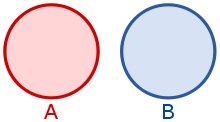
\includegraphics[width=0.8\linewidth]{./images/MGWI/220px-Disjunkte_Mengen} \end{center}
\end{column}
\end{columns}


\begin{Beispiele}[]

\begin{itemize}
\tightlist
\item
  Die Mengen \(A = \{1, 2, 3\}\) und \(B = \{7, 8, 11\}\) sind disjunkt,
  weil sie kein gemeinsames Element haben.
\item
  Die Mengen \(A = \{1, 2, 7\}\) und \(B = \{6, 7, 8, 11\}\) sind nicht
  disjunkt, da sie das Element \(7\) gemeinsam haben.
\end{itemize}

\end{Beispiele}

\end{frame}

\begin{frame}{Familie disjunkter Mengen}
\protect\hypertarget{familie-disjunkter-mengen}{}

\begin{columns}[T]
\begin{column}{0.66\textwidth}

\begin{definition}[Familie disjunkter Mengen]

Eine \textbf{Familie von Mengen} \(\displaystyle M_1,M_2, ... , M_n\)
ist eine \textbf{disjunkte Mengenfamilie}, falls Mengen
\textbf{paarweise disjunkt} sind; wenn also gilt:

\[ M_i \cap M_j = \emptyset \quad \text{ für } \!\,i \ne j \text{ und } 1 \leq i,j \leq n \]

\end{definition}
\end{column}

\begin{column}{0.33\textwidth}
\begin{center}
\includegraphics[width=0.6\linewidth]{./images/MGWI/126px-Disjuct-sets} \end{center}
\end{column}
\end{columns}


\begin{Beispiele}[]

\begin{itemize}
\tightlist
\item
  Die drei Mengen \(A = \{1, 2, 3\}\), \(B = \{4, 5\}\) und
  \(C = \{6, 7\}\) sind \emph{paarweise disjunkt}. \(A\), \(B\), \(C\)
  bilden also eine \emph{disjunkte Mengenfamilie}.
\item
  Die drei Mengen \(A = \{1, 2, 3\}\), \(B = \{4, 5\}\) und
  \(C = \{5, 6, 7\}\) sind \emph{nicht paarweise disjunkt}, da zumindest
  eine der drei möglichen Schnittmengen (nämlich \(B \cap C\)) nicht
  leer ist.
\end{itemize}

\end{Beispiele}

\end{frame}

\begin{frame}{Partition /\thinspace{}Zerlegung einer Menge}
\protect\hypertarget{partition-zerlegung-einer-menge}{}


\begin{definition}[Partiton oder Zerlegung einer Menge]

Gilt für eine Menge \(A\) und ihre \emph{nichtleeren}, \emph{paarweise
disjunkten} echten Teilmengen \(A_1, \dots, A_n\), dass
\(A = A_1 \cup A_2 \cup \cdots \cup A_n\) ist. So nennen wir die Mengen
\(A_1, \dots A_n\) eine \textbf{Zerlegung} oder auch \textbf{Partition
von \(A\)}.

\end{definition}


\begin{Beispiele}[]

\begin{itemize}
\tightlist
\item
  Für \(A= \{1,2,3,4,5,6,7,8\}\) bilden \(A_1=\{1,3,5,7\}\),
  \(A_2=\{2,8\}\) und \(A_3=\{4,6\}\) eine \emph{Partition}, denn
  \(A=A_1\cup A_2 \cup A_3\) und \(A_1 \cap A_2=\emptyset\),
  \(A_1 \cap A_3=\emptyset\) sowie \(A_2 \cap A_3=\emptyset\).
\item
  Für jede (nichtleere) Menge \(A\) bildet eine nichtleere, echte
  Teilmenge \(B\) und deren Komplement \(B^c\) eine \emph{Partition von
  \(A\)}.
\item
  Die drei Mengen \(A = \{1, 2, 3\}\), \(B = \{4, 5\}\) und
  \(C = \{5, 6, 7\}\) sind \emph{nicht paarweise disjunkt}, da
  \(B \cap C \neq \emptyset\).
\item
  Die folgende Aufzählung definierte eine (unendliche) disjunkte
  Mengenfamilie, die eine Partition der ganzen Zahlen darstellt:
  \(\{0\}, \{1, -1\}, \{2, -2\}, \{3, -3\}, \{4, -4\}, \ldots\).
\end{itemize}

\end{Beispiele}

\end{frame}

\begin{frame}{Übung 4:}
\protect\hypertarget{ubung-4}{}

\begin{enumerate}
[a)]
\item
  Geben Sie zur Menge \(A=\{1,2,3,4\}\) alle möglichen Partitionen mit
  genau zwei Mengen an.
\item
  Für die natürlichen Zahlen \(\mathbf{N}\) kann man mit
  \(U=\left\{x \,|\, x=2 \cdot n-1 \text{ mit } n \in \mathbf{N}\right\}\)
  und \(G = \mathbf{N} \setminus U\) eine Partion bilden. Geben Sie eine
  Definition von \(G\) ohne \(U\) zu benutzen an und bezeichnen Sie die
  beiden Mengen \(U\) und \(G\) sinnvoll.
\end{enumerate}

\note{\begin{enumerate}
[a)]
\item
  Es gibt die folgenden Partinition von \(M\) mit genau zwei Mengen:

  \begin{enumerate}
  [1)]
  \tightlist
  \item
    \(\left\{\{1\}, \{2, 3, 4\}\right\}\)
  \item
    \(\left\{\{2\}, \{1, 3, 4\}\right\}\)
  \item
    \(\left\{\{3\}, \{1, 2, 4\}\right\}\)
  \item
    \(\left\{\{4\}, \{1, 2, 3\}\right\}\)
  \item
    \(\left\{\{1,2\}, \{3, 4\}\right\}\)
  \item
    \(\left\{\{1,3\}, \{2, 4\}\right\}\)
  \item
    \(\left\{\{1,4\}, \{2, 3\}\right\}\)
  \end{enumerate}
\item
  \begin{itemize}
  \tightlist
  \item
    \(G = \left\{ x \,|\, x = 2\cdot n \text{ mit } n \in \mathbf{N}\right\}\),
  \item
    \(U\) ist die \emph{Menge der ungeraden natürlichen Zahlen},
  \item
    \(G\) ist die \emph{Menge der geraden natürlichen Zahlen}.
  \end{itemize}
\end{enumerate}}

\end{frame}

\begin{frame}{Die Potenzmenge}
\protect\hypertarget{die-potenzmenge}{}


\begin{definition}[Potenzmenge]

Die Menge aller Teilmengen einer Menge \(X\) heißt \textbf{Potenzmenge
von \(X\)} und ist eine Menge. Wir schreiben dafür:

\[ \mathcal{P}(X) := \left\{ U \,|\, U \subset X \right\} \]

\end{definition}


\begin{Beispiele}[]

\begin{enumerate}       
    \item $\displaystyle\mathcal{P}(\emptyset) = \{ \emptyset \}$
        
    \item $\displaystyle\mathcal{P}(\{ a \}) = \{ \emptyset, \{ a \} \}$
        
    \item $\displaystyle\mathcal{P}(\{ a, b \}) = \{ \emptyset, \{ a \}, \{ b \}, \{ a, b \} \}$
        
    \item $\displaystyle\mathcal{P}(\{ a, b, c \}) = \{ \emptyset, \{ a \}, \{ b \}, \{ c \}, \{ a, b \}, \{ a, c \}, \{ b, c \}, \{ a, b, c \} \}$
\end{enumerate}

\end{Beispiele}

\end{frame}

\begin{frame}{Übung 5:}
\protect\hypertarget{ubung-5}{}

\begin{enumerate}
[a)]
\tightlist
\item
  Bilden Sie die Potenzmenge von \(A=\{7,3,6\}\).
\item
  Die Menge \(M\) hat \(n\) Elemente. Wie viele Elemente hat die
  Potenzmenge?
\end{enumerate}

\note{\begin{enumerate}
[a)]
\tightlist
\item
  \(\displaystyle\mathcal{P}(A) = \{ \emptyset, \{7\}, \{ 3 \}, \{ 6 \}, \{ 7, 3 \}, \{ 7, 6 \}, \{ 3, 6 \}, \{ 7, 3, 6 \} \}\)
\item
  \(\displaystyle|\mathcal{P}(M)| = 2^n\)
\end{enumerate}}

\end{frame}

\hypertarget{exkurs-zahlenmengen}{%
\subsection{Exkurs: Zahlenmengen}\label{exkurs-zahlenmengen}}

\begin{frame}{Zahlen}
\protect\hypertarget{zahlen}{}


\begin{columns}[T]
	\begin{column}[t]{0.74\textwidth}

In seiner Schrift \glqq Was sind und was sollen Zahlen?\grqq\xspace 
schrieb Richard Dedekind 1888:

\vspace*{1.2em}

\begin{quote}
Die Zahlen sind freie Schöpfungen des menschlichen Geistes, sie dienen
als Mittel, um die Verschiedenheit der Dinge leichter und schärfer
aufzufassen. Durch den rein logischen Aufbau der Zahlenwissenschaft und
durch das in ihr gewonnene stetige Zahlenreich sind wir erst in den
Stand gesetzt, unsere Vorstellungen von Raum und Zeit genau zu
untersuchen, indem wir dieselben auf dieses in unserem Geiste
geschaffene Zahlenreich beziehen.
\end{quote}


	\end{column}
	\begin{column}[t]{0.24\textwidth}
\personDB{Dedekind}
	\end{column}
\end{columns}

\end{frame}

\begin{frame}{Natürliche Zahlen}
\protect\hypertarget{naturliche-zahlen}{}

Die Menge der \textbf{natürlichen Zahlen}

\begin{equation*}
        \mathbf{N} := \{1,2,3,4,5,...\}
\end{equation*}

\begin{center}
        \begin{tikzpicture}
              \draw[->] (1,0) -- (5.5,0) node [above] {$\mathbf{N}$};
              \foreach \x in {1,...,5}
                \draw (\x,0.1) -- (\x,-0.1) node [below] {\x};
            \foreach \x in {1,...,5}
                \filldraw[ball color=red!80,shading=ball] (\x, 0) circle  (0.06cm);
        \end{tikzpicture}
\end{center}

Wollen wir die natürlichen Zahlen statt bei \(1\) mit \(0\) beginnen
lassen, so schreiben wir \(\mathbf{N_0}\) für
\(\mathbf{N} \cup \{ 0 \}\).

\begin{center}
        \begin{tikzpicture}
              \draw[->] (0,0) -- (5.5,0) node [above] {$\mathbf{N_0}$};
              \foreach \x in {0,...,5}
                \draw (\x,0.1) -- (\x,-0.1) node [below] {\x};
            \foreach \x in {0,...,5}
                \filldraw[ball color=red!80,shading=ball] (\x, 0) circle  (0.06cm);
        \end{tikzpicture}
\end{center}

\end{frame}

\begin{frame}{Abzählbare Menge /\thinspace{}Peano-Axiome}
\protect\hypertarget{abzahlbare-menge-peano-axiome}{}

\begin{columns}[T]
\begin{column}{0.74\textwidth}
{\small{}

\textbf{Peano-Axiome}

\begin{enumerate}[(1)]
    \item   Die $1$ ist eine natürliche Zahl. 
    \item   Zu jeder natürlichen Zahl $n$ gibt es genau 
            einen \textit{Nachfolger} $n'$, der ebenfalls eine 
            natürliche Zahl ist. 
    \item   Es gibt keine natürliche Zahl, deren Nachfolger $1$ ist.
    \item   Jede natürliche Zahl ist Nachfolger höchstens einer 
            natürlichen Zahl. 
    \item   \textit{[Induktionsprinzip]}\, 
            Von allen Mengen $X$, welche 
            \begin{itemize}
                \item   die Zahl $1$ und 
                \item   mit jeder natürlichen Zahl $n$ auch stets 
                        deren Nachfolger $n'$ enthalten, 
            \end{itemize}
            ist die \textit{Menge der natürlichen Zahlen} die kleinste.
\end{enumerate}

}
\end{column}

\begin{column}{0.24\textwidth}
\personDB{Peano}
\end{column}
\end{columns}

\end{frame}

\begin{frame}{Von Neumanns Modell der natürlichen Zahlen}
\protect\hypertarget{von-neumanns-modell-der-naturlichen-zahlen}{}

\begin{columns}[T]
\begin{column}{0.74\textwidth}
{\footnotesize{}

\textbf{Mengentheoretisches Modell}

\begin{alignat*}{3}
    0 &:=    &&\quad\ \emptyset&&\\
    1 &:= 0' &&= \{0\}          &&= \{ \emptyset \}\\
    2 &:= 1' &&= \{0, 1\}       &&= \{ \emptyset, \{ \emptyset \} \}\\
    3 &:= 2' &&= \{0, 1, 2\}    &&= \{ \emptyset, \{ \emptyset \}, \{ \emptyset, \{ \emptyset \} \} \}\\
      &\vdots&& &&\\
    n'&:=    &&\quad\ \{0,1,\ldots,n\} &&= n \cup \{n\}
\end{alignat*}

}
\end{column}

\begin{column}{0.24\textwidth}
\personDB{vonNeumann}
\end{column}
\end{columns}


\begin{Bemerkung}[]

John von Neumann ist eine der bemerkenswertesten Personen des 20.
Jahrhunderts. Ich empfehle Ihnen die Arte Dokumentation
\href{http://www.sefiroth.net/MfWInf/videos/JohnVonNeumann.mp4}{John von
Neumann - Der Denker des Computer-Zeitalters}!

\end{Bemerkung}

\end{frame}

\begin{frame}{Übung 6:}
\protect\hypertarget{ubung-6}{}

Schreiben Sie die folgenden Zahlen in der von Neumann Darstellung

(also nur mit \(\emptyset\), \(\{\) und \(\}\)) :

\begin{align*}
    (a) & \quad 4 \\
    (b) & \quad 5 \\
    \intertext{ Welche Zahl verbirgt sich hinter: } \\
    (c) & \quad \left\{ \emptyset, \{ \emptyset \}, \{ \emptyset, \{ \emptyset \} \}, \{ \emptyset, \{ \emptyset \}, \{ \emptyset, \{ \emptyset \} \}\} \right\} \\
    (d) & \quad \left\{ \left\{ \right\}, \left\{ \left\{ \right\} \right\}, \left\{ \left\{ \right\}, \left\{ \left\{ \right\} \right\} \right\} \right\}
\end{align*}

\note{\begin{enumerate}
[a)]
\tightlist
\item
  \(4 = \{ \emptyset, \{ \emptyset \}, \{ \emptyset, \{ \emptyset \} \}, \{ \emptyset, \{ \emptyset \}, \{ \emptyset, \{ \emptyset \} \} \} \}\)
\item
  \(5 = \{ \emptyset, \{ \emptyset \}, \{ \emptyset, \{ \emptyset \} \}, \{ \emptyset, \{ \emptyset \}, \{ \emptyset, \{ \emptyset \} \} \}, \{ \emptyset, \{ \emptyset \}, \{ \emptyset, \{ \emptyset \} \}, \{ \emptyset, \{ \emptyset \}, \{ \emptyset, \{ \emptyset \} \} \} \} \}\)
\item
  \(4\)
\item
  \(3\)
\end{enumerate}}

\end{frame}

\begin{frame}{Die Gleichmächtigkeit von Mengen}
\protect\hypertarget{die-gleichmachtigkeit-von-mengen}{}

\begin{columns}[T]
\begin{column}{0.66\textwidth}

\begin{definition}[Gleichmächtigket von Mengen]

Man nennt zwei Mengen \textbf{gleichmächtig}, falls es eine
\emph{ein-ein-deutige} bzw. \emph{bijektive} Abbildung von der einen
Menge in die andere Menge gibt.

\end{definition}
\end{column}

\begin{column}{0.33\textwidth}
\begin{center}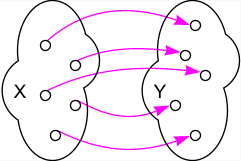
\includegraphics[width=0.7\linewidth]{./images/MGWI/Bijektivitaet_Mengenwolke} \end{center}
\end{column}
\end{columns}


\begin{Beispiele}[]

Es seien die Mengen \(A=\{1,2,3\}\) und \(B=\{a,b,c\}\) gegeben.

\begin{itemize}
\item
  \(A\) und \(B\) sind wegen der bijektiven Abbildung
  \(1 \leftrightarrow a\), \(2 \leftrightarrow b\),
  \(3 \leftrightarrow c\) \emph{gleichmächtig}.
\item
  Da Abbildungen ``nur in die Mengen gucken'' folgt sofort, dass die
  Menge \(C=\{1,2,3,1,2,3,1,2,3\}\) ebenfalls \emph{gleichmächtig} zu
  \(C\) und \(B\) ist.
\item
  Gleichmächtigkeit ist \textbf{transitiv},
  \mbox{d.\thinspace{}h.}\xspace{} \(C\) ist auch \emph{gleichmächtig}
  zu \(A\), da \(B\) zu beiden (\(A\) und \(C\)) gleichmächtig ist!
\end{itemize}

\end{Beispiele}

\end{frame}

\begin{frame}{Die Mächtigkeit von Mengen}
\protect\hypertarget{die-machtigkeit-von-mengen}{}


\begin{definition}[Mächtigkeit von Mengen /\thinspace{}Anzahl der
Elemente]

Ist eine Menge \(A\) \emph{gleichmächtig} zu einer natürlichen Zahl
\(n\) (im Sinne von Neumanns), so nennen wir die Menge \textbf{endlich}.

Wir setzen in diesem Fall dann\\
\[ \#A := |A| := n \] und sprechen von der \emph{Anzahl der Elemente}
von \(A\) oder dem \textbf{Betrag} von \(A\).

\end{definition}


\begin{Fakt}[]

Ist eine Menge endlich, so entspricht der \emph{Betrag} der \emph{Anzahl
der unterscheidbaren Elemente} der Menge.

\end{Fakt}


\begin{Beispiel}[]

\(\#\{1, 2, 3, 4\} = \#\{1, 1, 2, 3, 3, 3, 4\} = |\{1, 2, 2, 3, 3, 3, 3, 3, 3, 3, 3, 4\}| = |\{1, 2, 3, 4\}| = 4\)

\end{Beispiel}

\end{frame}

\begin{frame}{Unendlichkeit von Mengen}
\protect\hypertarget{unendlichkeit-von-mengen}{}


\begin{definition}[Mächtigkeitsbegriffe von Mengen]

Ist die Menge \emph{gleichmächtig} zu \ldots{}

\begin{itemize}
\tightlist
\item
  \ldots{} der Menge der natürlichen Zahlen selbst, so nennen wir die
  Menge \textbf{abzählbar unendlich};
\item
  \ldots{} einer Teilmenge der natürlichen Zahlen, so nennen wir die
  Menge \textbf{abzählbar};
\end{itemize}

Gibt es eine echte Teilmenge der Menge, zu der die Menge selbst
\emph{gleichmächtig} ist, so nennen wir die Menge
\textbf{(Dedekind-)unendlich}.

\end{definition}

\end{frame}

\begin{frame}{Mächtigkeit von Potenzmengen}
\protect\hypertarget{machtigkeit-von-potenzmengen}{}


\begin{Satz}[Satz von Cantor]

\begin{itemize}
\tightlist
\item
  Für \emph{endliche Mengen} \(X\) gilt: \begin{equation*}
        |\mathcal{P}(X)| = 2^{|X|}
    \end{equation*}
\item
  Für (endliche und) \emph{unendliche Mengen} \(X\) gilt (der Satz von
  Cantor): \begin{equation*}
        |X| < |\mathcal{P}(X)|
    \end{equation*}
\end{itemize}

\end{Satz}


\begin{Beispiele}[]

\begin{itemize}
\tightlist
\item
  Ist \(A=\{a\}\), so ist \textbar{}A\textbar{}= 1. Mit
  \(\mathcal{P}(A)=\{\emptyset, \{a\}\}\) ist \begin{equation*}
        |\mathcal{P}(A)|=2 = 2^1 = 2^{|A|}.
    \end{equation*}
\item
  \(|\mathbf{N}| < |\mathcal{P}(\mathbf{N})|\).
\end{itemize}

\end{Beispiele}

\end{frame}

\begin{frame}{Die vollständige Induktion}
\protect\hypertarget{die-vollstandige-induktion}{}

Das 5. Axiom von Peano bildet die Grundlage für das \emph{Beweisprinzip}
der \textbf{vollständigen Induktion}.

Seit \emph{Richard Dedekind} ist die \textbf{vollständige Induktion}
folgendermaßen festgelegt:


\begin{definition}[vollständige Induktion]

Um zu beweisen, dass eine Aussage \(A(n)\) für alle natürlichen Zahlen
\(n \geq m\) gilt, genügt es zu zeigen, dass sie für :

\begin{itemize}
\tightlist
\item
  \(n = m\) gilt, also \(A(m)\) gilt und
\item
  dass aus der Gültigkeit der Aussage für eine Zahl \(n \geq m\) stets
  auch die Gültigkeit\\
  für die folgende Zahl \(n+1\) folgt. (\(A(n) \Longrightarrow A(n+1)\))
\end{itemize}

\end{definition}

\begin{center}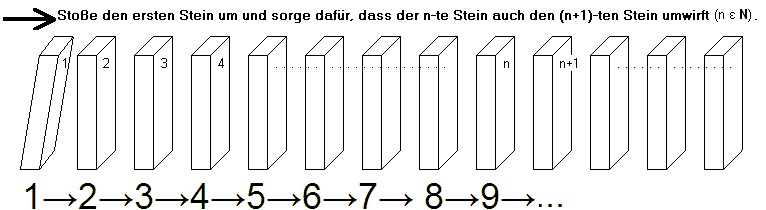
\includegraphics[width=0.6\linewidth]{./images/MGWI/Domino} \end{center}

{\tiny{}

Quelle: \href{http://tinyurl.com/op2rhse}{``Domino - 2'' von Joachim
Mohr - Eigenes Werk.}{]}

Lizenziert unter CC BY-SA 3.0 über Wikimedia Commons

}

\end{frame}

\begin{frame}{Die vollständige Induktion}
\protect\hypertarget{die-vollstandige-induktion-1}{}

Wir führen die vollständige Induktion in zwei Schritten durch:

\begin{enumerate}
\item
  \glqq \textbf{Induktionsanfang}\grqq
\item
  \glqq \textbf{Induktionsschritt}\grqq

  \begin{itemize}
  \tightlist
  \item
    \glqq \textit{Induktionsannahme}\grqq
  \item
    \glqq \textit{Induktionsschluss}\grqq
  \end{itemize}
\end{enumerate}

\end{frame}

\begin{frame}{Beispiel für eine vollständige Induktion}
\protect\hypertarget{beispiel-fur-eine-vollstandige-induktion}{}


\begin{columns}[T]
	\begin{column}[t]{0.74\textwidth}


\begin{Satz}[von Maurolicus (1575)]

Die Summe aller ungeraden Zahlen von \(1\) bis \((2n-1)\) ist gleich dem
Quadrat von \(n\).

Genauer gesagt:

Es gilt \[ 1 + 3 + 5 + \cdots + (2n-1) = n^2 \] für alle natürlichen
Zahlen \(n\).

\end{Satz}


	\end{column}
	\begin{column}[t]{0.24\textwidth}
\personDB{Maurolicus}
	\end{column}
\end{columns}


\begin{Uebung}[]

Testen Sie die Vermutung mit den folgenden Werten \(n=3\), \(4\) und
\(5\)!

\end{Uebung}

\end{frame}

\begin{frame}{Beispiel für eine vollständige Induktion}
\protect\hypertarget{beispiel-fur-eine-vollstandige-induktion-1}{}


\begin{Beweis}[des Satzes von Maurolicus]

Wir zeigen \(1 + 3 + 5 + \cdots + (2n-1) = n^2\) mit Hilfe der
\textbf{vollständigen Induktion}: \small

\begin{description}
        \item[\glqq Induktionsanfang\grqq] ($n=1$):
            $\displaystyle 1 = 1^2 $  
        \item[\glqq Induktionsschritt\grqq] ($n \Longrightarrow n+1$):
        
            \begin{itemize}
                \item[\glqq Ind.-annahme \grqq]
                    Es gelte $\displaystyle 1+3+5+\cdots + (2n-1) =n^2$.  
                \item[\glqq Ind.-schluss\grqq]  
            Zu zeigen ist dann, dass
            $\displaystyle 1+3+5+\cdots + (2n-1) + (2[n+1]-1) =[n+1]^2$
            gilt.  
            \begin{align*}
                1+3+5+ &\cdots + (2n-1) + (2[n+1]-1)
                        = n^2 + 2 [n+1] -1 \\
                        &= n^2 + 2n + 2 -1
                        = \underbrace{n^2 +2 n +1}_{\text{1. Binomische Formel}}
                        = (n+1)^2. \\
            \end{align*}
            \end{itemize}
\end{description}

\end{Beweis}


\begin{Bemerkung}[Video gefällig?]

\begin{itemize}
\tightlist
\item
  \href{https://youtu.be/y8B8fl_usm0}{Beweis des Satzes von Maurolicus
  als Video!}
\end{itemize}

\end{Bemerkung}

\end{frame}

\begin{frame}{Die Menge der ganzen Zahlen}
\protect\hypertarget{die-menge-der-ganzen-zahlen}{}

Die Menge der \textbf{ganzen Zahlen} ist

\[ \mathbf{Z} := \{0, -1, 1, -2, 2, -3, 3,...\} = \{...,-3,-2,-1,0,1,2,3,...\} \]

\begin{center}
        \begin{tikzpicture}
              \draw[<->] (-5.5,0) -- (5.5,0) node [above] {$\mathbf{Z}$};
              \foreach \x in {-5,...,5}
                \draw (\x,0.1) -- (\x,-0.1) node [below] {\x};
            \foreach \x in {-5,...,5}
                \filldraw[ball color=red!80,shading=ball] (\x, 0) circle  (0.06cm);
        \end{tikzpicture}
\end{center}


\begin{Bemerkung}[]

Die Menge der ganzen Zahlen ist gleichmächtig zur Menge der natürlichen
Zahlen!

\end{Bemerkung}

\end{frame}

\begin{frame}{Übung 7: Summen}
\protect\hypertarget{ubung-7-summen}{}

Beweisen Sie jeweils mit Hilfe der vollständigen Induktion die folgenden
Aussagen:

\begin{enumerate}
[a)]
\item
  \(\displaystyle \sum_{k=1}^n (2k) = n\cdot(n+1)\) für alle
  \(n \geq 1\)
\item
  \emph{Gauß'sche Summenformel}:

  \(\displaystyle \sum_{k=1}^n k = \frac{n \cdot (n+1)}{2}\) für alle
  \(n \geq 1\)
\item
  \emph{Geometrische Summenformel}:

  \(\displaystyle \sum_{k=0}^n q^k = \frac{1-q^{n+1}}{1-q}\) für alle
  \(q \ne 1\) und \(n \geq 0\)
\end{enumerate}

\note{}

\end{frame}

\begin{frame}{Übung 8: Produkte}
\protect\hypertarget{ubung-8-produkte}{}

Beweisen Sie jeweils mit Hilfe der vollständigen Induktion die folgenden
Aussagen:

\begin{enumerate}
[a)]
\tightlist
\item
  \(\displaystyle \prod^n_{k=2} \left(1-\frac{2}{k\cdot (k+1)}\right) = \frac{1}{3} \cdot \left(1+\frac{2}{n}\right)\)
  für alle \(n \geq 2\)
\item
  \(\displaystyle \prod^n_{k=1} 4^k = 2^{n \cdot (n+1)}\)
\item
  \(\displaystyle \left(1-\frac{1}{2}\right) \cdot \left(1-\frac{2}{3}\right) \cdot \left(1-\frac{3}{4}\right) \cdot \cdots \cdot \left(1-\frac{n-1}{n}\right) = \frac{1}{n!}\)
  für alle \(n\geq 2\)
\end{enumerate}

\note{}

\end{frame}

\begin{frame}{Übung 9: Ungleichungen}
\protect\hypertarget{ubung-9-ungleichungen}{}

Beweisen Sie mit Hilfe der vollständigen Induktion die folgenden
Ungleichungen:

\begin{enumerate}
[a)]
\tightlist
\item
  \(\displaystyle 2^n > n+1\) für alle \(n \geq 2\)
\item
  \(\displaystyle 2^n > n^2\) für alle \(n \geq 5\)
\item
  \(\displaystyle 2^n > n^3\) für alle \(n \geq 10\)
\item
  \(\displaystyle n! > 2^n\) für alle \(n \geq 4\)
\end{enumerate}

\note{}

\end{frame}

\begin{frame}{Übung 10: Finde den Fehler I/II}
\protect\hypertarget{ubung-10-finde-den-fehler-iii}{}

\textbf{Behauptung:} Alle ungeraden Zahlen sind durch 2 teilbar.

\textbf{Beweis:} Sei \(n\) die \(n\)-te ungerade Zahl, welche durch 2
teilbar ist. Die \((n+1)\)-te ungerade Zahl ist dann \(n+2\) ist damit
eine Summe aus zwei durch 2 teilbaren Summanden und damit wieder durch 2
teilbar. Aus der vollständigen Induktion folgt, dass alle ungeraden
Zahlen durch 2 teilbar sind.

\end{frame}

\begin{frame}{Übung 11: Finde den Fehler II/II}
\protect\hypertarget{ubung-11-finde-den-fehler-iiii}{}

\textbf{Behauptung:} Es passen unendlich viele Sandkörner in einen LKW.

\textbf{Induktionsanfang:} Da ein Sandkorn sehr klein ist, passt auf
jeden Fall ein Sandkorn in einen LKW.

\textbf{Induktionsschritt:} Gehen wir davon aus, dass \(n\) Sandkörner
im LKW sind. Da ein Sandkorn sehr, sehr klein ist im Vergleich zum
Laderaum eines LKWs, passt ein zusätzliches Sandkorn auf jeden Fall in
den LKW rein. Damit passen auch \(n+1\) Sandkörner in einen LKW.

Daraus folgt, es passen beliebig viele Sandkörner in einen LKW.

\end{frame}

\begin{frame}{Die Menge der rationalen Zahlen}
\protect\hypertarget{die-menge-der-rationalen-zahlen}{}

Die Menge der \textbf{rationalen Zahlen}

\begin{equation*}
        \mathbf{Q} := \left\{ \left.\frac{q}{p} \, \right| \, q \in \mathbf{Z}, p \in \mathbf{N}, p \text{ und } q \text{ sind teilerfremd} \right\}
\end{equation*}


\begin{Bemerkung}[]

Die Menge der rationalen Zahlen ist gleichmächtig zur Menge der
natürlichen Zahlen!

(vgl.: \href{http://tinyurl.com/p2k6u7f}{Cantors erstes
Diagonalargument})

\end{Bemerkung}

\end{frame}

\begin{frame}{Die Menge der irrationalen Zahlen}
\protect\hypertarget{die-menge-der-irrationalen-zahlen}{}

Die Menge der \textbf{irrationalen Zahlen} besteht aus \emph{reellen
Zahlen}, die nicht als Bruch zweier ganzer Zahlen dargestellt werden
kann.

\begin{equation*}
    \mathbf{I} := \left\{ x \in \mathbf{R}\, \left|\, \text{es gibt keine } p, q \in\mathbf{Z} \text{ mit } x = \frac{p}{q} \text{ und } q \neq 0 \right. \right\}
\end{equation*}


\begin{Bemerkungen}[]

\begin{itemize}
\item
  Im Gegensatz zu rationalen Zahlen, die als endliche oder periodische
  Dezimalzahlen dargestellt werden können, sind irrationale Zahlen
  solche, deren Dezimaldarstellung nicht abbricht und nicht periodisch
  ist.
\item
  Es gibt zwei Typen von Irrationalzahlen:

  \begin{itemize}
  \tightlist
  \item
    \emph{algebraische Zahlen} (etwa quadratische Wurzeln aus
    Nicht-Quadratzahlen, \mbox{z.\thinspace{}B.}\xspace{} \(\sqrt{2}\),
    oder auch \(1+\sqrt[3]{5}\)),
  \item
    \emph{transzendente Zahlen} (etwa die Kreiszahl
    \(\pi = 3{,}14159\dots\) oder auch die Eulersche Zahl
    \(e = 2{,}71828\dots\)).
  \end{itemize}
\end{itemize}

\end{Bemerkungen}

\end{frame}

\begin{frame}{Reelle Zahlen}
\protect\hypertarget{reelle-zahlen}{}

Die Menge der \textbf{reellen Zahlen} ist

\[ \mathbf{R} = \mathbf{Q} \cup \mathbf{I}\]

\begin{center}
    \begin{tikzpicture}
        \draw[<->] (-5.5,0) -- (5.5,0) node [above] {$\mathbf{R}$};
        \foreach \x in {-5,...,5}
                    \draw (\x,0.1) -- (\x,-0.1) node [below] {\x};
        \draw[color=red] (-5.5,0) -- (5.5,0);
    \end{tikzpicture}
\end{center}


\begin{Bemerkung}[]

Die Menge der reellen Zahlen ist \textbf{nicht} gleichmächtig zur Menge
der natürlichen Zahlen!

(vgl.:

\begin{itemize}
\tightlist
\item
  \href{http://tinyurl.com/p83fezm}{Cantors zweites Diagonalargument}
  und
\item
  \href{http://bit.ly/1MlpAa8}{Cantors erster Überabzählbarkeitsbeweis}
\end{itemize}

)

\end{Bemerkung}

\end{frame}

\begin{frame}{Positive und negative Zahlen}
\protect\hypertarget{positive-und-negative-zahlen}{}


\begin{definition}[Zur Erinnerung]

\begin{itemize}
\tightlist
\item
  Wir nennen eine Zahl \(x\) mit \(x > 0\) \textbf{positiv}.
\item
  Wir sprechen bei \(x < 0\) von einer \textbf{negativen} Zahl \(x\).
\item
  Die Zahl \(0\) ist weder \emph{positiv} noch \emph{negativ}!
\item
  Für \(x \geq 0\) sagen wir, dass \(x\) \textbf{nicht negativ} ist und
  sprechen bei \(x \leq 0\) von einer \textbf{nicht positiven} Zahl.
\item
  Die Menge der \emph{positiven reellen Zahlen} bezeichnen wir als
  \begin{equation*}
        \mathbf{R}^+ \text{  oder  }\mathbf{R}^{>0}.
    \end{equation*}
\item
  Für die Menge der \emph{nicht negativen ganzen Zahlen} schreiben wir
  \begin{equation*}
        \mathbf{Z}^{\geq 0} = \mathbf{N}_0. 
    \end{equation*}
\end{itemize}

\end{definition}

\end{frame}

\begin{frame}{Der Betrag}
\protect\hypertarget{der-betrag}{}


\begin{definition}[(Absolut-)Betrag einer Zahl]

Für eine beliebige reelle Zahl \(x\), ist der \textbf{Betrag} definiert
als \begin{equation*}
        |x| := \begin{cases}
                    x   &: x \geq 0 \\
                    -x  &: x < 0
                \end{cases}
\end{equation*}

\end{definition}


\begin{Beispiele}[]

\begin{equation*}
        |-6|      = -(-6)     = 6,   \qquad 
        |4|       = 4,    \qquad 
        |0|       = 0,    \qquad 
        |-a|      = |a|,
\end{equation*}

\begin{equation*}
    | x-5 | =   \begin{cases}
                    x-5             &: x \geq 5 \\
                    -(x-5)=-x+5     &: x < 5
                \end{cases}
\end{equation*}

\end{Beispiele}

\end{frame}

\hypertarget{mengen-als-abstrakte-datenstruktur}{%
\subsection{Mengen als abstrakte
Datenstruktur}\label{mengen-als-abstrakte-datenstruktur}}

\begin{frame}{Mengen in Progammiersprachen}
\protect\hypertarget{mengen-in-progammiersprachen}{}

Die Idee der Menge (aus der Mathematik) ist als abstrakte Datenstruktur
in der Informatik bekannt.

Einige Porgrammiesprachen unterstützen dieses Konzept:

\begin{itemize}
\item
  \textbf{Java} \footnote<.->{vgl.
    \url{http://openbook.rheinwerk-verlag.de/javainsel9/javainsel_13_005.htm\#mj45263b87fd44c62f2cde668164897a93}}
  etwa mit dem Interface \emph{java.util.Set} und den Implementierungen
  \emph{java.util.HashSet}, \emph{LinkedHashSet}, \emph{EnumSet},
  \emph{CopyOnWriteArraySet} und \emph{java.util.TreeSet}.
\item
  \textbf{Python} \footnote<.->{vgl.
    \url{https://www.python-kurs.eu/python3_sets_mengen.php}} mit dem
  Datentyp \emph{set}.
\item
  \textbf{R} \footnote<.->{vgl.
    \url{https://www.rdocumentation.org/packages/sets/versions/1.0-18/topics/set}}
  mit dem Paket \emph{sets}.
\end{itemize}

\end{frame}

\begin{frame}[fragile]{Python I/III}
\protect\hypertarget{python-iiii}{}

Erstellen von Mengen in \emph{Python}:

\begin{Shaded}
\begin{Highlighting}[]
\NormalTok{A }\OperatorTok{=} \BuiltInTok{set}\NormalTok{([}\DecValTok{1}\NormalTok{,}\DecValTok{2}\NormalTok{,}\DecValTok{3}\NormalTok{]) }\CommentTok{# Menge via constructor}
\NormalTok{B }\OperatorTok{=} \BuiltInTok{set}\NormalTok{([}\DecValTok{2}\NormalTok{,}\DecValTok{3}\NormalTok{])}
\NormalTok{C }\OperatorTok{=}\NormalTok{ \{}\DecValTok{3}\NormalTok{,}\DecValTok{4}\NormalTok{,}\DecValTok{5}\NormalTok{\} }\CommentTok{# Menge via '\{' , '\}'}
\end{Highlighting}
\end{Shaded}

Differenz von Mengen

\begin{Shaded}
\begin{Highlighting}[]
\NormalTok{A }\OperatorTok{=}\NormalTok{ \{}\DecValTok{1}\NormalTok{,}\DecValTok{2}\NormalTok{,}\DecValTok{3}\NormalTok{\} }
\NormalTok{B }\OperatorTok{=}\NormalTok{ \{}\DecValTok{2}\NormalTok{,}\DecValTok{3}\NormalTok{\}  }
\CommentTok{# Mengendiffferenz A \textbackslash{} B:}
\NormalTok{A.difference(B)  }\CommentTok{# \{1\}}
\NormalTok{A}\OperatorTok{-}\NormalTok{B  }\CommentTok{# \{1\}}
\end{Highlighting}
\end{Shaded}

\end{frame}

\begin{frame}[fragile]{Python II/III}
\protect\hypertarget{python-iiiii}{}

Schnitt zweier Mengen

\begin{Shaded}
\begin{Highlighting}[]
\NormalTok{A }\OperatorTok{=}\NormalTok{ \{}\DecValTok{1}\NormalTok{,}\DecValTok{2}\NormalTok{,}\DecValTok{3}\NormalTok{\}}
\NormalTok{C }\OperatorTok{=}\NormalTok{ \{}\DecValTok{3}\NormalTok{,}\DecValTok{4}\NormalTok{,}\DecValTok{5}\NormalTok{\} }
\CommentTok{# Schnittmenge von A und C:}
\NormalTok{A.intersection(C)  }\CommentTok{# \{3\}}
\NormalTok{A }\OperatorTok{&}\NormalTok{ C  }\CommentTok{# \{3\}}
\end{Highlighting}
\end{Shaded}

Vereinigung zweier Mengen

\begin{Shaded}
\begin{Highlighting}[]
\NormalTok{A }\OperatorTok{=}\NormalTok{ \{}\DecValTok{1}\NormalTok{,}\DecValTok{2}\NormalTok{,}\DecValTok{3}\NormalTok{\}}
\NormalTok{C }\OperatorTok{=}\NormalTok{ \{}\DecValTok{3}\NormalTok{,}\DecValTok{4}\NormalTok{,}\DecValTok{5}\NormalTok{\}}
\CommentTok{# Vereinigungsmenge von A und C}
\NormalTok{A.union(C)  }\CommentTok{# \{1, 2, 3, 4, 5\}}
\NormalTok{A }\OperatorTok{|}\NormalTok{ C }\CommentTok{#  \{1, 2, 3, 4, 5\}}
\end{Highlighting}
\end{Shaded}

\end{frame}

\begin{frame}[fragile]{Python III/III}
\protect\hypertarget{python-iiiiii}{}

Teilmengen

\begin{Shaded}
\begin{Highlighting}[]
\NormalTok{A }\OperatorTok{=}\NormalTok{ \{}\DecValTok{1}\NormalTok{,}\DecValTok{2}\NormalTok{,}\DecValTok{3}\NormalTok{\}}
\NormalTok{C }\OperatorTok{=}\NormalTok{ \{}\DecValTok{1}\NormalTok{,}\DecValTok{2}\NormalTok{,}\DecValTok{3}\NormalTok{,}\DecValTok{4}\NormalTok{\}}
\CommentTok{# Teilmengenbeziehungen:}
\NormalTok{A.issubset(C)  }\CommentTok{# True}
\NormalTok{A }\OperatorTok{<}\NormalTok{ C  }\CommentTok{# True }
\NormalTok{A }\OperatorTok{<=}\NormalTok{ C  }\CommentTok{# True}
\NormalTok{C }\OperatorTok{<}\NormalTok{ A  }\CommentTok{# False}
\NormalTok{C }\OperatorTok{<=}\NormalTok{ A  }\CommentTok{# False}
\NormalTok{A }\OperatorTok{<}\NormalTok{ A  }\CommentTok{# False}
\NormalTok{A }\OperatorTok{<=}\NormalTok{ A  }\CommentTok{# True}
\end{Highlighting}
\end{Shaded}

Elemente

\begin{Shaded}
\begin{Highlighting}[]
\NormalTok{A }\OperatorTok{=}\NormalTok{ \{}\DecValTok{1}\NormalTok{,}\DecValTok{2}\NormalTok{,}\DecValTok{3}\NormalTok{\}}
\CommentTok{# Prüfung ob Element der Menge:}
\DecValTok{1} \KeywordTok{in}\NormalTok{ A  }\CommentTok{# True}
\DecValTok{4} \KeywordTok{in}\NormalTok{ A  }\CommentTok{# False}
\end{Highlighting}
\end{Shaded}

\end{frame}

\hypertarget{mengenlehre-fortsetzung}{%
\subsection{Mengenlehre (Fortsetzung)}\label{mengenlehre-fortsetzung}}

\begin{frame}{Übung 12:}
\protect\hypertarget{ubung-12}{}

Gegeben sind die Mengen \begin{align*}
    A &= \{ 1,2,3,4,5,6,7,8,9\} \\
    B &= \{ n \in \mathbf{N} \,|\, n \leq 4 \} \\
    C &= \{ n \in \mathbf{N} \,|\, n \text{ gerade} \} \\
    D &= \{ n \in \mathbf{N} \,|\, n \text{ ist ungerade und } n \leq 11 \}
\end{align*}

Bestimmen Sie: \(A \cup B\), \(A \setminus B\), \(B \setminus A\),
\(C \cap D\), \(A \cap D\), \(C \setminus D\), \(D \setminus C\)

\note{}

\end{frame}

\begin{frame}{Übung 13:}
\protect\hypertarget{ubung-13}{}

Seien die Mengen \(A = \{a, b, c, d\}\), \(B=\{a, c, g\}\) und
\mbox{$C=\{c, g, m, n,p\}$} gegeben.

Bestimmen Sie:

\begin{enumerate}
[a)]
\item
  \(A \cup B\) b) \(A \cup C\) c) \(B \cup C\) d) \(A \cap B\) e)
  \(A \cap C\)
\item
  \(B \cap C\) g) \(A \cup (B \cup C)\) h) \((A \cap B) \cup C\) i)
  \((A \cup B) \cap C\) k) \((A \cap B) \cup (A \cap C)\)
\item
  \(A \setminus B\) m) \(C \setminus (B \setminus A)\) n)
  \((C \setminus B) \setminus A\)
\end{enumerate}

\end{frame}

\begin{frame}{Rechengesetze für Mengen}
\protect\hypertarget{rechengesetze-fur-mengen}{}

Für je zwei Mengen \(A\) und \(B\) gelten die folgenden Sätze:

\begin{columns}[T]
\begin{column}{0.49\textwidth}

\begin{Satz}[Absorptionsgesetz]

\(A \cap (A \cup B) = A\) und \(A \cup (A \cap B) = A\)

\end{Satz}


\begin{Satz}[vom Widerspruch]

\((A\setminus B) \cap B = \emptyset\)

\end{Satz}
\end{column}

\begin{column}{0.49\textwidth}

\begin{Satz}[v. ausgeschlossenen 3.]

\((A \setminus B) \cup B = A \cup B\)

\end{Satz}


\begin{Satz}[Die Regeln von de Morgan]

\((A \cup B)^c = A^c \cap B^c\) und \((A \cap B)^c = A^c \cup B^c\)
\footnote<.->{Vgl. \href{http://www.bibleserver.com/text/EU/3.Mose11}{3.
  Mose Kapitel 11} oder \href{http://islam.de/13827.php?sura=5}{Sure 5
  Vers 1 und 3}}

\end{Satz}
\end{column}
\end{columns}

\end{frame}

\begin{frame}{Das geordnete Paar /\thinspace{}Produktmenge}
\protect\hypertarget{das-geordnete-paar-produktmenge}{}

Nehmen wir zwei Mengen, z.,B. \(A=\{1,2,3\}\) und \(B=\{2,3,5\}\).
Bilden wir nun aus den Elementen von \(A\) und \(B\) \emph{neue}
Elemente derart, dass wir jeweils \(x\) aus \(A\) mit einem Element
\(y\) aus \(B\) zu einem \textbf{geordneten Paar} (oder auch
\textbf{Tuppel}) \((x; y)\) zusammenfassen, so erhalten wir eine
\textbf{Produktmenge}:

\[ A \times B   = \{ (1;\, 2), (2;\, 2), (3;\, 2), (1;\, 3), (2;\, 3), (3;\, 3), (1;\, 5), (2;\, 5), (3;\, 5) \} \]

Die Elemente von \(A \times B\) sind nicht mehr einzelne Zahlen, sondern
\emph{geordnete} Zahlen\emph{paare}. Das Paar \((2;\, 3)\) ist vom Paar
\((3;\, 2)\) verschieden!


\begin{definition}[Geordnetes Paar]

Wahlweise via \((x, y) = \{ x, \{x, y\}\}\) oder
\((x, y) = \{ \{\emptyset, x\}, \{y\}\}\)

\end{definition}

\end{frame}

\begin{frame}{Das cartesische Produkt}
\protect\hypertarget{das-cartesische-produkt}{}

Allgemein definieren wir somit:


\begin{definition}[Produktmenge]

Unter der \textbf{Produktmenge} (dem \textbf{cartesischem Produkt}, der
\textbf{Paarmenge}) \(A \times B\) (gelesen \glqq A kreuz B\grqq)
versteht man die \emph{Menge aller geordneten Paar} \((x;\, y)\) mit der
Eigenschaft \(x \in A\) und \(y \in B\):

\[  A \times B := \left\{ (x; \, y) \,|\, x \in A \text{ und } y \in B \right\}. \]

Noch allgemeiner ist
\[ A_1 \times A_2 \times \dots \times A_n := \left\{ (x_1;\, x_2; \dots;\, x_n) \,|\, x_i \in A_i \text{ für } i=1,2, \dots, n \right\} \]

\end{definition}


\begin{Bemerkung}[]

Ist \(A_1=A_2=\cdots=A_n=A\), so schreiben wir kurz \(A^n\) für
\(A_1 \times A_2 \times \dots \times A_n\).

\end{Bemerkung}

\end{frame}

\begin{frame}{Übung 14:}
\protect\hypertarget{ubung-14}{}

Für die Mengen \(A=\{a, b, c\}\) und \(B=\{d, e\}\) bilden Sie die
folgenden Produktmengen:

\begin{enumerate}
[a)]
\tightlist
\item
  \(\displaystyle A \times B\)
\item
  \(\displaystyle A^2\)
\item
  \(\displaystyle B \times A \times B\)
\item
  \(\displaystyle A \times B \times A\)
\end{enumerate}

\note{}

\end{frame}

\begin{frame}{Exkurs: Kreuzprodukt als typisches Datenbankproblem}
\protect\hypertarget{exkurs-kreuzprodukt-als-typisches-datenbankproblem}{}

\emph{Kreuzprodukte} treten in \emph{relationalen Datenbanken} auf. Die
Gründe dafür sind meistens:

\begin{itemize}
\tightlist
\item
  fehlende Spezifizierung des Zusammenhanges der Tabellen
\item
  fehlerhafte Formulierung der Abfrage
\end{itemize}

\end{frame}

\begin{frame}{Exkurs: Kreuzprodukt als typisches Datenbankproblem}
\protect\hypertarget{exkurs-kreuzprodukt-als-typisches-datenbankproblem-1}{}


\begin{Beispiel}[]

\small

Nehmen wir folgende Tabellen an:

\vspace*{1em}

\begin{columns}
        \begin{column}{5cm}
            \begin{tabular}{|l|l|l|}
                \hline
                \multicolumn{3}{|l|}{{\it\bf Mitarbeiter}} \\
                \hline
                {\bf MA-ID} & {\bf Vorname} & {\bf Name} \\
                \hline
                MA1 & Hans  & Meier \\
                \hline
                MA2 & Helga & Müller    \\
                \hline
                \vdots & \vdots & \vdots \\
                \hline
                MA50 & Osman & Öztürk \\
                \hline
            \end{tabular}
        \end{column}
        \begin{column}{5cm}
            \begin{tabular}{|l|l|l|}
                \hline
                \multicolumn{3}{|l|}{{\it\bf Adressen}} \\
                \hline
                {\bf AD-ID} & {\bf Strasse} & {\bf PLZ} \\
                \hline
                AD1 & Kaiserstra{\ss}e 1    & 45123 \\
                \hline
                AD2 & Königsweg 2   & 45454 \\
                \hline
                \vdots & \vdots & \vdots \\
                \hline
                AD30 & Heldenallee 99 & 44444 \\
                \hline
            \end{tabular}
        \end{column}
\end{columns}

\vspace*{1em}

Eine \emph{SQL-Abfrage} wie:

\vspace*{0.5em}

\texttt{ \textbf{select} (Name, Strasse, PLZ) \textbf{from} Mitarbeiter, Adressen;  }

\vspace*{0.5em}

liefert das Kreuzprodukt der beiden Tabellen ,,und somit \(1\,500\)
Datensätze!

Abhilfe schafft hier eine \emph{eineindeutige Zuordnung} von
Mitarbeitern und Adressen.\\
\mbox{($\to$ \textit{Relationen})}

\end{Beispiel}

\end{frame}

\hypertarget{kombinatorik-oder-die-kunst-des-zahlens}{%
\section{Kombinatorik oder die Kunst des
Zählens}\label{kombinatorik-oder-die-kunst-des-zahlens}}

\begin{frame}{Was ist Kombinatorik?}
\protect\hypertarget{was-ist-kombinatorik}{}

Die \textbf{Kombinatorik} ist ein Teilgebiet der Mathematik, welches
sich mit der Bestimmung der Anzahl von möglichen \emph{Anordnungen} oder
\emph{Auswahlen} von

\begin{itemize}
\tightlist
\item
  \emph{unterscheidbaren} oder \emph{nicht unterscheidbaren} Objekten
\item
  \emph{mit} oder \emph{ohne} Beachtung der \emph{Reihenfolge}
\end{itemize}

beschäftigt.

In der Mathematik finden sich einige Anwendungen für die Kombinatorik:

\begin{itemize}
\tightlist
\item
  Bestimmung der Anzahl von Teilmengen
\item
  Bestimmung der Größe von Mengen \mbox{(z.\thinspace{}B.}\xspace{} der
  Potenzmenge)
\item
  Berechnung von Wahrscheinlichkeiten (sofern alle Ereignisse gleich
  Wahrscheinlich sind)
\end{itemize}

\end{frame}

\begin{frame}{Was ist Kombinatorik?}
\protect\hypertarget{was-ist-kombinatorik-1}{}

Ein paar Beispiele für die Frage nach der Anzahl:

\begin{itemize}
\tightlist
\item
  Wie viele und welche Möglichkeiten gibt es aus 12 Personen 2er-Teams
  zu bilden?
\item
  Wie viele und welche Fälle sind zu beachten, wenn ein Objekt, durch
  zwei Eigenschaften gekennzeichnet ist, von denen eine vier und die
  andere drei Ausprägungen haben kann?
\item
  Wie viele Passworte kann man bilden, wenn das Passwort 6-8 Zeichen
  lang ist und mindestens eine Ziffer enthält?
\end{itemize}

\end{frame}

\begin{frame}{Beziehung Kombinatorik zur Wahrscheinlichkeitsrechnung}
\protect\hypertarget{beziehung-kombinatorik-zur-wahrscheinlichkeitsrechnung}{}

Mit Hilfe der Kombinatorik werden Wahrscheinlichkeiten abgeleitet.

Dabei wir mit der Kombinatorik die Anzahl der
gesuchten/guten/gewünschten Ereignisse ins Verhältnis zur Gesamtzahl der
Ereignisse gesetzt.


\begin{Beispiele}[für die Frage nach der (abgeleiteten)
Wahrscheinlichkeit]

\begin{itemize}
\tightlist
\item
  Wir groß ist die Wahrscheinlichkeit einen Sechser im Lotto zu
  erreichen? (Und mit Superzahl?)
\item
  Wie groß ist die Wahrscheinlichkeit, dass auf einer Feier zwei
  Personen am gleichen Tag (im Jahr) Geburtstag haben?
\end{itemize}

\end{Beispiele}

\end{frame}

\begin{frame}{Zur Erinnerung}
\protect\hypertarget{zur-erinnerung-1}{}


\begin{definition}[Gleichmächtigkeit]

Seien \(A\) und \(B\) zwei Mengen. Wir sagen \(A\) ist
\textbf{gleichmächtig} zu \(B\), wenn es eine \emph{bijektive} Abbildung
\(f:\, A \to B\) gibt.

In diesem Fall schreiben wir \(|A|= |B|\) (oder auch \(\#A = \#B\)).

\end{definition}


\begin{definition}[endliche Mengen und deren Elementanzahl]

Ist eine Menge \(A\) gleichmächtig mit einer \emph{natürlichen Zahl} --
wie sie \emph{von Neumann} definiert hat --, so schreiben wir auch

\begin{equation*}
    |A| = n,\quad \text{ für ein } n \in \mathbf{N}
\end{equation*}

und nennen die Menge \textbf{endlich}.

\end{definition}

\end{frame}

\begin{frame}{Zur Erinnerung}
\protect\hypertarget{zur-erinnerung-2}{}


\begin{Beispiel}[Von Neumann und Gleichmächtigkeit]

Die Menge \(A=\{x, y, z\}\) ist gleichmächtig zur Menge
\(3=\{ \emptyset, \{ \emptyset \}, \{ \emptyset, \{ \emptyset \} \} \}\),
denn:

\begin{itemize}
\tightlist
\item
  \(\displaystyle x \leftrightarrow \emptyset\),
\item
  \(\displaystyle y \leftrightarrow \{ \emptyset \}\),
\item
  \(\displaystyle z \leftrightarrow \{ \emptyset, \{ \emptyset \} \}\)
\end{itemize}

Darum schreiben wir auch \(|A|=3\) mit der \emph{natürlichen Zahl} 3 und
sagen:

\begin{itemize}
\tightlist
\item
  Die Menge \(A\) hat \(3\) Elemente.
\end{itemize}

\end{Beispiel}


\begin{definition}[Abzählbare Mengen]

Jede Menge, die gleichmächtig zu \(\mathbf{N}\) oder einem Element aus
\(\mathbf{N}\) ist, nennen wir \textbf{abzählbar}.

\end{definition}

\end{frame}

\begin{frame}{Summenregel für endliche Mengen}
\protect\hypertarget{summenregel-fur-endliche-mengen}{}

\small


\begin{Satz}[Summenregel (für endliche Mengen)]

Für beliebige Mengen \(A\) und \(B\) gilt:\vspace*{-.5em}
\begin{equation*} 
    |A \cup B| = |A| + |B| - |A \cap B| 
\end{equation*}

Ist \(A \cap B = \emptyset\), so gilt:\vspace*{-.5em} \begin{equation*} 
    |A \cup B| = |A| + |B| 
\end{equation*}

\small

\end{Satz}


\begin{Beispiel}[Kurze Wörter]

Die Anzahl aller Wörter die aus drei Kleinbuchstaben bestehen und mit
einem Vokal (a,e,i,o,u) anfangen oder enden ist:\vspace*{-.5em}
\begin{equation*}
    5 \cdot 26^2 + 26^2 \cdot 5 - 5 \cdot 26 \cdot 5 = 6\,110
\end{equation*}

\end{Beispiel}


\begin{Beispiel}[Mengen]

Sei \(A=\{a, b, c, d\}\) und \(B=\{x, y, z\}\). Dann ist:\vspace*{-.5em}
\begin{equation*}
    |A|=4,\, |B|=3,\, |A \cup B|= |A| + |B| = 7\text{, da }|A \cap B| = 0
\end{equation*}

\end{Beispiel}

\end{frame}

\begin{frame}{Einstufiger Auswahl-/Entscheidungsprozess}
\protect\hypertarget{einstufiger-auswahl-entscheidungsprozess}{}

\small

Die Summenformel bestimmt die Anzahl der Alternativen, die in einer
einfachen Entscheidung gewählt werden können. Wenn die unterschiedlichen
Mengen von Alternativen, die berücksichtigt werden, Schnittmengen
aufweisen, sollen deren Elemente nur einfach berücksichtigt werden.


\begin{Uebung}[Übung]

Mailing-Aktion eines Versandhauses:

\begin{itemize}
\tightlist
\item
  \(A=\)\{Menge aller Besteller/innen, die in den letzten vier Wochen
  bestellt haben\}
\item
  \(B=\)\{Menge aller Besteller/innen von Haushaltsartikeln\}
\item
  \(C=\)\{Menge aller Bestellerinnen\}
\end{itemize}

Wie viele Mails werden versendet, wenn an alle Kunden, die zumindest zu
einer der Mengen gehören, berücksichtigt werden?

\textbf{Tipp:} Skizzieren Sie die Situation mit Hilfe eines
Mengendiagramms!

\end{Uebung}

\end{frame}

\begin{frame}{Prinzip von Inklusion und Exklusion}
\protect\hypertarget{prinzip-von-inklusion-und-exklusion}{}

Die \emph{Summenregel} liefert für zwei Mengen \(A\) und \(B\) die
Formel:\vspace*{-1.5em} \begin{equation*}
    |A \cup B| = |A| + |B| - |A \cap B|
\end{equation*} Für drei Mengen \(A\), \(B\), \(C\) erhalten
wir:\vspace*{-1.5em}

\begin{columns}[T]
\begin{column}{0.6\textwidth}
\begin{align*}
    |A \cup B \cup C|   &= |A| + |B| + |C| \\
                        &\phantom{=} - |A \cap B| - |A \cap C| - |B \cap C| \\
                        &\phantom{=} + |A \cap B \cap C|
\end{align*}
\end{column}

\begin{column}{0.4\textwidth}
\begin{center}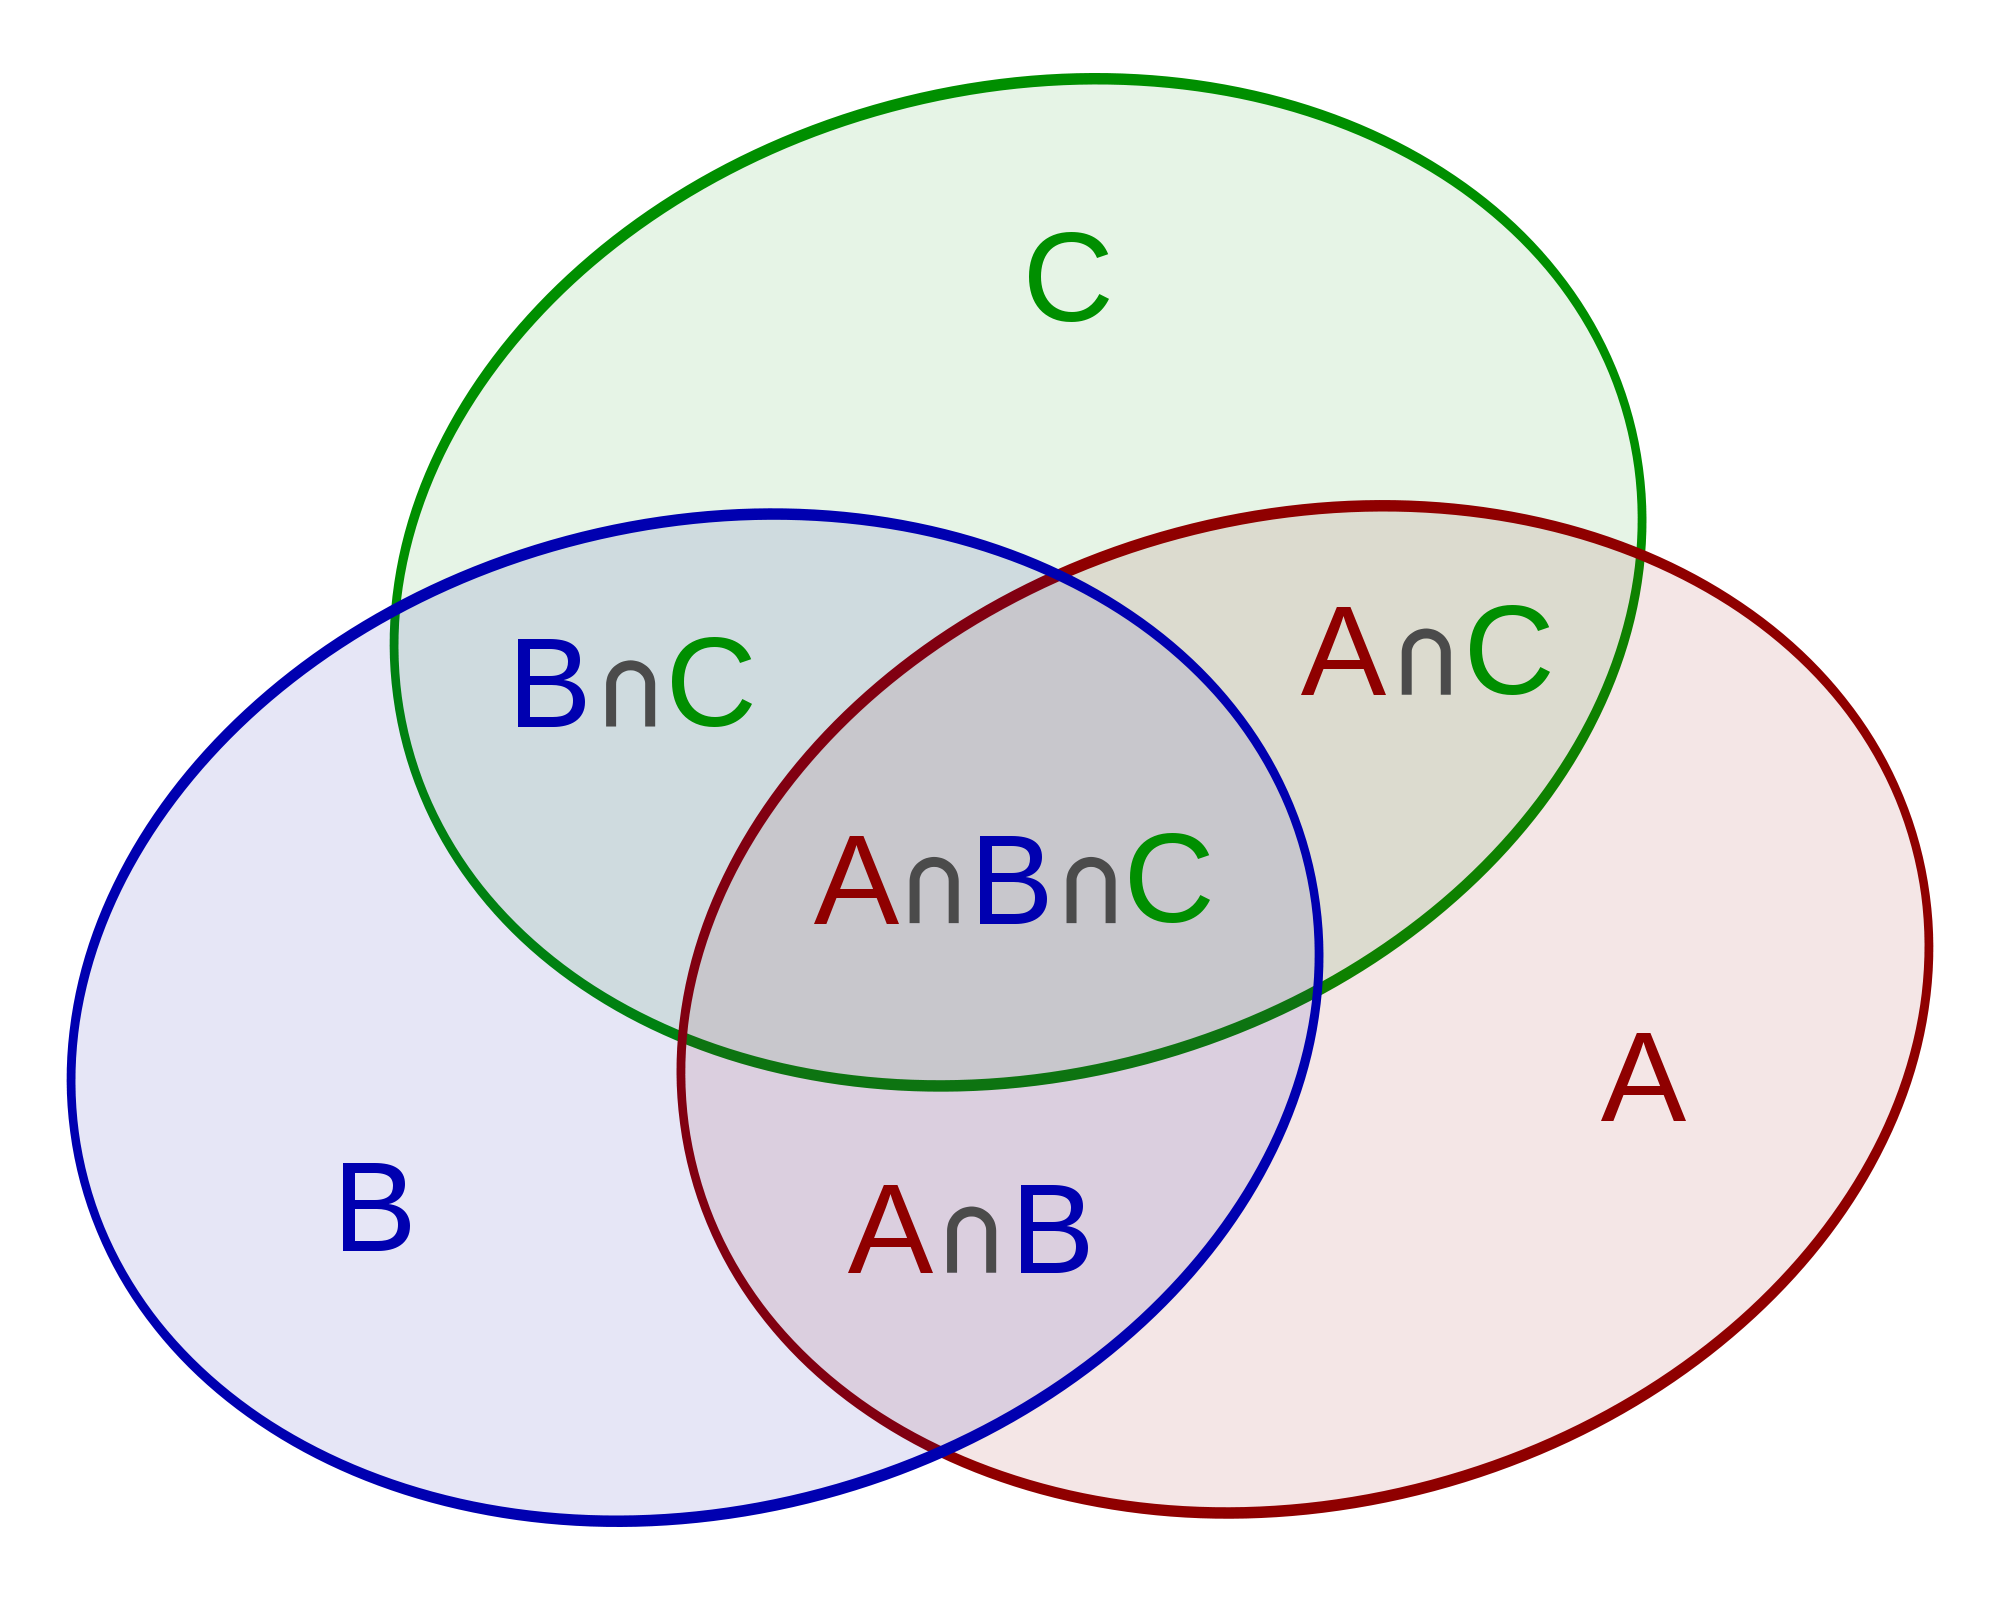
\includegraphics[width=0.55\linewidth]{./images/MGWI/2000px-Inclusion-exclusion} \end{center}
\end{column}
\end{columns}

\vspace*{-0.7em}


\begin{Satz}[Prinzip von Inklusion und Exklusion]

Sei \(X = \bigcup_{i=1}^n A_i\) eine \emph{endliche Menge} die sich als
eine Vereinigung von \(n\) Teilmengen \(A_1,A_2, \ldots, A_n\) schreiben
lässt. Zu einer \emph{Indexmenge} \(I \subseteq \{1,2,\ldots,n\}\) sei
\(A_I:= \bigcap_{i \in I} A_i\) der Schnitt über alle durch die Elemente
der Indexmenge bezeichneten Teilmengen, wobei \(A_\emptyset = X\)
entspricht. Dann gilt \begin{equation*}
    |X| = \sum_{\emptyset \not= I \subseteq \{1,\ldots,n\}} \left( -1\right)^{|I|+1}|A_I|~.
\end{equation*}

\end{Satz}

\end{frame}

\begin{frame}{Produktregel für endliche Mengen}
\protect\hypertarget{produktregel-fur-endliche-mengen}{}


\begin{Satz}[Produktregel (für endliche Mengen)]

Für beliebige Mengen \(A\) und \(B\) gilt:\vspace*{-.7em}
\begin{equation*} 
    |A \times B| = |A| \cdot |B| 
\end{equation*}

\end{Satz}


\begin{Beispiel}[Routenplanung]

Herr Besserwisser will von Berlin nach Dortmund.

\begin{itemize}
\tightlist
\item
  Für die Strecke von Berlin nach Hannover kennt er 5 Routen.
\item
  Für die Strecke Hannover nach Dortmund ist er mit 3 Routen vertraut.
\end{itemize}

Wie viele Möglichkeiten hat Herr Besserwisser von Berlin über Hannover
nach Dortmund zu fahren?

Die Entscheidung erfolgt in zwei \emph{unabhängigen} Schritten:

\begin{itemize}
\tightlist
\item
  \textbf{1. Schritt:} Entscheidung für die Route von Berlin nach
  Hannover aus den fünf Möglichkeiten.
\item
  \textbf{2. Schritt:} Die Tour von Hannover nach Dortmund hat drei
  Optionen.
\end{itemize}

Insgesamt also \(5 \cdot 3 = 15\) mögliche Routen.

\end{Beispiel}

\end{frame}

\begin{frame}{Produktregel für mehr als zwei Mengen}
\protect\hypertarget{produktregel-fur-mehr-als-zwei-mengen}{}


\begin{Satz}[Produktregel]

Sei \(k\in\mathbf{N}\) und \(A_1,\dots,A_k\) Mengen. Dann gilt:

\begin{equation*} 
    \left| A_1 \times A_2 \times \cdots \times A_k\right| = \prod_{i=1}^{k} \left| A_i \right| 
\end{equation*}

\end{Satz}


\begin{Bemerkung}[In Worten:]

Die Mächtigkeit des kartesischen Produktes mehrerer Mengen ist gleich
dem Produkt der Mächtigkeit des Einzelmengen.

\end{Bemerkung}


\begin{Beispiel}[Kurze Wörter]

Die Anzahl der Wörter der Länge 3 aus Kleinbuchstaben und Ziffern, die
mit einem Buchstaben anfangen ist: \begin{equation*}
    26 \cdot 36 \cdot 36 = 33\,696
\end{equation*}

\end{Beispiel}

\end{frame}

\begin{frame}{Beispiel:}
\protect\hypertarget{beispiel}{}

{\small{}


\begin{Beispiel}[Einfache Passworte aus 6-8 Zeichen]

Eine Anwendung der Summen- und Produktregel ist die Anzahl aller
Passwörter mit 6-8 Zeichen zu bestimmen.

\begin{itemize}
\tightlist
\item
  Da die Schnittmenge der Passworte mit 6, 7 oder 8 Zeichen leer ist,
  können die Mächtigkeiten der Mengen addiert werden.
\item
  Die Anzahl der Möglichkeiten, die \(n\)-te Stelle im Passwort zu
  belegen, ist \emph{unabhängig} von den Belegungen der vorangehenden
  Stellen.
\end{itemize}

Also können wir die Anzahl der Möglichkeiten multiplizieren.

\begin{itemize}
\item
  Die Anzahl der möglichen Passworte hängt nur vom Zeichenvorrat ab.
\item
  Nehmen wir an, dass nur Großbuchstaben zulässig sind,
  \mbox{d.\thinspace{}h.}\xspace{} es gibt 26 Zeichen.
\end{itemize}

Somit ist\vspace*{-1.8em} \begin{align*}
    |\{\text{6-stellige Passworte}\}| = 26^6 &= \phantom{208}\,308\,915\,776, \\
    |\{\text{7-stellige Passworte}\}| = 26^7 &= \phantom{20}8\,031\,810\,176, \\
    |\{\text{8-stellige Passworte}\}| = 26^8 &= 208\,827\,064\,576.\\[.4em]
\text{Die Anzahl insgesamt ist also \hfil} 26^6+ 26^7+ 26^8  &=217\,167\,790\,528.
\end{align*}

\end{Beispiel}

}

\end{frame}

\begin{frame}{Permutationen}
\protect\hypertarget{permutationen}{}


\begin{definition}[(\(k\)-)Permutation, Variation]

Eine Auswahl von \(k\) Objekten aus einer Menge von \(n\) Elementen, bei
der \emph{die Reihenfolge eine Rolle spielt}, nennt man
\textbf{geordnete Auswahl} (auch \textbf{Variation} oder
\textbf{\(k\)-Permutation}).

Der Spezialfall \(k=n\), bei dem alle Elemente ausgewählt und angeordnet
werden, heißt \textbf{Permutation}.

\end{definition}


\begin{Beispiele}[Permutationen]

\begin{itemize}
\item
  Der Sektion Ringen des Sportvereins mit \(12\) Ringern macht einen
  internen Wettkampf. Wie viele Möglichkeiten gibt es für die Besetzung
  des ersten, zweiten und dritten Platzes?
\item
  Wie viele Möglichkeiten gibt es, \(5\) Bücher auf einem Regalbrett
  anzuordnen?
\end{itemize}

\end{Beispiele}

\end{frame}

\begin{frame}{Kombination}
\protect\hypertarget{kombination}{}


\begin{definition}[Kombination]

Eine Auswahl von \(k\) Objekten aus einer Menge von \(n\) Elementen
\emph{ohne Beachtung der Reihenfolge}, nennt man \textbf{ungeordnete
Auswahl} oder \textbf{Kombination}.

\end{definition}


\begin{Beispiele}[Kombination]

\begin{itemize}
\item
  In der Sektion Ringen des Sportvereins mit 12 Mitgliedern soll in dem
  Turnier jedes Mitglied gegen jedes andere kämpfen.\\
  Wie viele Kämpfe sind notwendig?
\item
  \emph{Der Klassiker:} Wie viele Möglichkeiten gibt es, 6 Zahlen aus
  den natürlichen Zahlen von 1 bis 49 zu ziehen?
\end{itemize}

\end{Beispiele}

\end{frame}

\begin{frame}{Anzahl der Permutationen}
\protect\hypertarget{anzahl-der-permutationen}{}

Gegeben ist die Menge \(A=\{a,b,c,d,e\}\).

Wie viele Möglichkeiten für 3-Permutationen aus \(A\) gibt es?

\begin{itemize}
\tightlist
\item
  Für die Ziehung des ersten Objekts gibt es 5 Möglichkeiten. Die
  verbleibende Menge hat 4 Elemente.
\item
  Für die Ziehung des zweiten Objekts gibt noch 4 Möglichkeiten. Es
  bleiben 3 Elemente zur Auswahl.
\item
  Für die Ziehung des dritten Objekts gibt noch 3 Möglichkeiten.
\end{itemize}

\end{frame}

\begin{frame}{Anzahl der Permutationen}
\protect\hypertarget{anzahl-der-permutationen-1}{}

Allgemein gilt:

Werden \(k\) Elemente aus einer Menge mit \(n\) Elementen unter
Beachtung der Reihenfolge (als \emph{\(k\)-Permutation}) gezogen, so
gibt es für die

\begin{tabular}{lcl}
        erste Ziehung   & $n$       & Alternativen \\  
        zweite Ziehung  & $(n-1)$   & Alternativen \\  
        dritte Ziehung  & $(n-2)$   & Alternativen \\  
        $\quad $\vdots  & \vdots    & Alternativen \\ 
        $k$-te Ziehung  & $(n-k+1)$ & Alternativen 
\end{tabular}

Die Anzahl der möglichen \(k\)-Permutationen ergibt sich durch
Multiplikation der Alternativen auf jeder Stufe des Ziehungsprozesses.

\end{frame}

\begin{frame}{Satz zur Anzahl der Permutationen}
\protect\hypertarget{satz-zur-anzahl-der-permutationen}{}


\begin{Satz}[Anzahl der Permutationen]

Die Anzahl der \(k\)-Permutationen aus einer Menge mit \(n\) Elementen
wird als \(P(n,k)\) bezeichnet und ist gegeben durch: \begin{equation*} 
    P(n,k)  = n \cdot (n-1) \cdot (n-2) \cdot \dots \cdot (n-k+1)   
            = \frac{n!}{(n-k)!} 
\end{equation*}

Man spricht hier auch von einer \textbf{geordneten Auswahl}.

Speziell gibt es

\begin{equation*} 
    P(n,n)  = n \cdot (n-1) \cdot (n-2) \cdot \dots \cdot 2 \cdot 1   
            = n! 
\end{equation*}

verschiedene Anordnungen der \(n\) Elemente.

\end{Satz}


\begin{Beispiel}[Traveling Salesman Problem]

Ein Geschäftsreisender besucht nacheinander \(n\) Orte. Dann gibt es
\(n!\) mögliche Reiserouten!

\end{Beispiel}

\end{frame}

\begin{frame}{Beispiel: Die Besetzung der Siegertreppe beim Ringkampf}
\protect\hypertarget{beispiel-die-besetzung-der-siegertreppe-beim-ringkampf}{}

Zwölf Ringer kämpfen um den ersten, zweiten und dritten Platz

\begin{itemize}
\item
  Für den ersten Platz gibt es zwölf Kandidaten
\item
  Ist der erste Platz vergeben, verbleiben 11 Kandidaten für Platz 2
\item
  Für den dritten Platz bleiben dann noch 10 Kandidaten
\end{itemize}

Damit ergeben sich \(12 \cdot 11 \cdot 10 = 1320\) Möglichkeiten, wie
das Siegerpodest besetzt sein kann.

Anwendung der Formel: \begin{align*}
    P(12,3) &= \frac{12!}{(12-3)!} \\ 
            &= \frac{1 \cdot 2 \cdot 3 \cdot \dots \cdot 9 \cdot 10 \cdot 11 \cdot 12}{1 \cdot 2 \cdot 3 \cdot \dots \cdot 9} \\
            &= 10 \cdot 11 \cdot 12 = 1320
\end{align*}

\end{frame}

\begin{frame}{Beispiel: Die Anordnung der Bücher}
\protect\hypertarget{beispiel-die-anordnung-der-bucher}{}

Fünf Bücher sind auf einem Regalbrett anzuordnen

\begin{itemize}
        \item   Mit jedem eingestellten Buch verringert sich die Anzahl 
                der Optionen für den nächsten Platz auf dem Brett um eins.
        \item   Für den fünften Platz existiert schließlich nur noch ein Buch.
\end{itemize}

Es gibt damit: \(1 \cdot 2 \cdot 3 \cdot 4 \cdot 5\) \(= 120\)
Möglichkeiten

\begin{align*}
        P(5,5)  &= \frac{5!}{(5-5)!} = 5! \qquad (\text{denn }0!=1) \\
                &= 1 \cdot 2 \cdot 3 \cdot 4 \cdot 5 = 120
\end{align*}

\end{frame}

\begin{frame}{Anzahl von Kombinationen}
\protect\hypertarget{anzahl-von-kombinationen}{}

Gegeben ist die Gruppe von Schachspielern \(S=\{a,b,c,d\}\).

Wie viele Möglichkeiten für zweier Gruppen von Spielern aus \(S\) gibt
es?

\begin{itemize}
\item
  Bekannt ist, dass es \(3 \cdot 4 = 12\) Möglichkeiten von Paarungen
  gibt, wenn die Reihenfolge eine Rolle spielt.
\item
  Da aber \mbox{z.\thinspace{}B.}\xspace{} \((a,b) = (b,a)\) ist, werden
  dabei alle zweier Gruppen doppelt gezählt.
\item
  Die Anzahl der geordneten Auswahlen ist also durch \(2\) zu teilen.
\end{itemize}

Folgende Paarungen ergeben sich:

\begin{equation*}
    \{a,b\}, \{a,c\}, \{a,d\}, \{b,c\}, \{b,d\}, \{c,d\}
\end{equation*}

\emph{Da bei den Kombinationen die Reihenfolge der Elemente keine
Bedeutung hat, können sie als Mengen angesehen werden.}

\end{frame}

\begin{frame}{Anzahl von Kombinationen}
\protect\hypertarget{anzahl-von-kombinationen-1}{}

Allgemein gilt:

Die Bestimmung der Anzahl der möglichen Kombinationen von \(k\)
Elementen aus einer Menge von \(n\) Elementen kann in zwei Schritte
zerlegt werden:

\begin{enumerate}
\tightlist
\item
  Die Anzahl der \(k\)-Permutationen ermittelt.
\item
  Diese Anzahl durch die Anzahl der Permutationen der \(k\) Elemente
  geteilt, da diese für die Kombination gleichwertig sind. Die Anzahl
  der Permutationen von \(k\) Elementen ist gegeben durch: \(k!\)
\end{enumerate}


\begin{Satz}[Anzahl von Kombinationen]

Die Anzahl der möglichen Kombinationen von \(k\) Elementen aus einer
Menge mit \(n\) Elementen wird als \(C(n,k)\) bezeichnet und ist gegeben
durch:

\begin{equation*} 
    C(n,k) = \frac{P(n,k)}{k!} = \frac{n!}{(n-k)!} \cdot \frac{1}{k!} = \frac{n!}{k!(n-k)!} 
\end{equation*}

Für \(k>n\) ist \(C(n,k) = 0\).

\end{Satz}

\end{frame}

\begin{frame}{Binomialkoeffizienten}
\protect\hypertarget{binomialkoeffizienten}{}


\begin{definition}[Binomialkoeffizienten]

Für zwei natürliche Zahlen \(n\) und \(k\) mit \(k \leq n\) heißt die
Zahl

\begin{equation*}
    \binom{n}{k} := \frac{n!}{k! \cdot (n-k)!}
\end{equation*}

der \textbf{Binomialkoeffizient $n$ über $k$}.

Für \(k>n\) ist der Binomialkoeffizient gleich Null.

\end{definition}


\begin{Beispiel}[Binomialkoeffizienten]

Berechnen Sie:

\begin{itemize}
\tightlist
\item
  \(\binom{5}{0}\), \(\binom{5}{1}\), \(\binom{5}{2}\),
  \(\binom{5}{3}\), \(\binom{5}{4}\) und \(\binom{5}{5}\)
\end{itemize}

\end{Beispiel}

\end{frame}

\begin{frame}{Rechenregeln für Binomialkoeffizienten}
\protect\hypertarget{rechenregeln-fur-binomialkoeffizienten}{}

Für Binomialkoeffizienten gelten die folgenden Regeln
(\(n,k \in \mathbf{N}\) und \(k \leq n\)):

\textbf{Wichtige Werte: (Randwerte)} \begin{equation*}
    \binom{n}{0} = \binom{n}{n} = 1
\end{equation*}

\textbf{Summe:} \begin{equation*}
    \binom{n}{1} = \binom{n}{n-1} =  \sum_{j=1}^{n-1} 1 = n
\end{equation*}

\textbf{Gauß'sche-Summen:} \begin{equation*}
    \binom{n}{2} = \binom{n}{n-2} = \sum_{j=1}^{n-1} j =  \frac{n\cdot(n-1)}{2}
\end{equation*}

\end{frame}

\begin{frame}{Rechenregeln für Binomialkoeffizienten (forts.)}
\protect\hypertarget{rechenregeln-fur-binomialkoeffizienten-forts.}{}

\textbf{Symmetrieeigenschaft:} \begin{equation*}
    \binom{n}{n-k} = \binom{n}{k} 
\end{equation*} \(\Longrightarrow\) Die Auswahl von \(k\) aus \(n\)
Objekten ist gleichbedeutend von der Bestimmung von \(n-k\) Objekten,
die nicht ausgewählt werden!

\textbf{Anzahl \textit{aller} Teilmengen einer $n$-elementigen Menge:}
\begin{equation*}
    \sum_{k=0}^{n} \binom{n}{k} = 2^n
\end{equation*}

\textbf{Additionseigenschaft:} \begin{equation*}
    \binom{n}{k} + \binom{n}{k+1} = \binom{n+1}{k+1} 
\end{equation*}

\end{frame}

\begin{frame}{Das Pascal'sche Dreieck}
\protect\hypertarget{das-pascalsche-dreieck}{}

\begin{columns}
        \begin{column}{0.74\textwidth}
            \begin{tabular}{ccccccccccccc}
                &   &   &   &   &   & 1 &   &   &   &   & \\  
                &   &   &   &   &   &   &   &   &   &   &   \\
                &   &   &   &   & 1 &   & 1 &   &   &   & \\  
                &   &   &   &   &   &   &   &   &   &   &   \\
                &   &   &   & 1 &   & 2 &   & 1 &   &   & \\  
                &   &   &   &   &   &   &   &   &   &   &   \\
                &   &   & 1 &   & 3 &   & 3 &   & 1 &   & \\  
                &   &   &   &   &   &   &   &   &   &   &   \\
                &   & 1 &   & 4 &   & 6 &   & 4 &   & 1 & \\
                &   &   &   &   &   &   &   &   &   &   &   \\
                & 1 &   & 5 &   & 10&   & 10&   & 5 &   & 1
            \end{tabular}
        \end{column}
        \begin{column}{0.24\textwidth}
            \personDB{Pascal}
        \end{column}
\end{columns}


\begin{Bemerkung}[]

Das Pascal'sche Dreieck war jedoch schon früher bekannt und wird deshalb
auch heute noch nach anderen \glqq Entdeckern\grqq\xspace benannt. In
China spricht man vom \textit{Yang-Hui-Dreieck}, in Italien vom
\textit{Tartaglia-Dreieck} und im Iran vom \textit{Chayy\={a}m-Dreieck}.

\end{Bemerkung}

\end{frame}

\begin{frame}{Erweiterung der binomischen Formeln}
\protect\hypertarget{erweiterung-der-binomischen-formeln}{}

\newcommand{\mycolor}{\color{blue}}

Es ist: \begin{align*}
        (a+b)^0 &= {\color{blue}1}\\
        (a+b)^1 &= {\color{blue}1 \cdot} a \; + {\color{blue}1 \, \cdot} \phantom{a}\;b\\
        (a+b)^2 &= {\color{blue}1 \cdot} a^2 + {\color{blue}2} \cdot a\;b + \phantom{0} {\color{blue}1 \, \cdot} \phantom{a}b^2\\ 
        (a+b)^3 &= {\color{blue}1 \cdot} a^3 + {\color{blue}3} \cdot a^2b + \phantom{0} {\color{blue}3}   \cdot a\;b^2 + \phantom{0}{\color{blue}1 \, \cdot} \,\phantom{a}b^3 \\ 
        (a+b)^4 &= {\color{blue}1 \cdot} a^4 + {\color{blue}4} \cdot a^3b + \phantom{0} {\color{blue}6}   \cdot a^2b^2 + \phantom{0}{\color{blue}4}   \cdot a\;b^3 + {\color{blue}1 \, \cdot}\phantom{a}b^4 \\
        (a+b)^5 &= {\color{blue}1 \cdot} a^5 + {\color{blue}5} \cdot a^4b +            {\color{blue}10}   \cdot a^3b^2 +            {\color{blue}10}   \cdot a^2b^3 + {\color{blue}5 \cdot}ab^4 + {\color{blue}1 \cdot}\phantom{a}b^5
\end{align*}

\end{frame}

\begin{frame}{Der binomische Lehrsatz}
\protect\hypertarget{der-binomische-lehrsatz}{}

\begin{columns}
    \begin{column}[t]{0.74\textwidth}
        \begin{Satz}[Newton's binomische Formeln]
            Für zwei (reelle) Zahlen $a$ und $b$ und eine natürliche Zahl $n$ gilt der \textbf{binomische Lehrsatz}:
            \begin{equation*}
                (a+b)^n = \sum_{k=0}^n {\color{blue} \binom{n}{k} }  a^{n-k}  b^k
            \end{equation*}
        \end{Satz}
    \end{column}
    \begin{column}[t]{0.24\textwidth}
    \vspace*{-1em}
    \personDB{Newton}
    \end{column}
\end{columns}

\small


\begin{Beispiel}[Potenzieren ohne Taschenrechner]

\vspace*{-0.5em}

\begin{align*}
    101^5   &= (100+1)^5 \\
            &= {\color{blue} 1} \cdot 100^0\cdot 1^5 + {\color{blue} 5} \cdot 100^1\cdot 1^4 + {\color{blue} 10} \cdot 100^2\cdot 1^3 + {\color{blue} 10} \cdot 100^3\cdot 1^2 + \\
            &\qquad + {\color{blue} 5} \cdot 100^4\cdot 1^1 + {\color{blue} 1} \cdot 100^5\cdot 1^0\\
            &= {\color{blue} 1} + {\color{blue} 5} 00 + {\color{blue} 10} 0\,000 + {\color{blue} 10} \,000\,000 + {\color{blue} 5} 00\,000\,000 + {\color{blue} 1} 0\,000\,000\,000 \\
            &= 10\,510\,100\,501
\end{align*}

\end{Beispiel}

\end{frame}

\begin{frame}{Wiederholte Verwendung der Objekte}
\protect\hypertarget{wiederholte-verwendung-der-objekte}{}

Elemente können in Kombinationen und Variationen der Grundgesamtheit
auch mehrfach vorkommen:

\begin{itemize}
        \item   Passworte können mehrfach identische Zeichen enthalten  
                (Reihenfolge ist bedeutsam)
        \item   Verteilung von Bonuspunkten auf mehrere Kandidaten  
                (Reihenfolge der Punktevergabe ist irrelevant)
\end{itemize}

Kann ein Objekt mehrfach verwendet werden, ändern sich die Zählregeln
der Kombinatorik

\begin{itemize}
        \item   Bei relevanter Reihenfolge Rückgriff auf die Produktregel  
                (Anzahl der Möglichkeiten pro Element wird multipliziert)
        \item   Bei irrelevanter Reihenfolge würde dies gleiche Ergebnisse
                mehrfach zählen
\end{itemize}

Man nennt das \textbf{Ziehung mit Zurücklegen}.

\end{frame}

\begin{frame}{Ziehung mit Zurücklegen ohne Beachtung der Reihenfolge}
\protect\hypertarget{ziehung-mit-zurucklegen-ohne-beachtung-der-reihenfolge}{}

Es können 4 Bonuspunkte auf 5 Kandidaten \((A, B, C, D, E)\) verteilt
werden.

Relevant ist nur die Anzahl der Punkte, die ein Kandidat erhält. Für
jede Punktvergabe gibt es 5 Optionen \((A, B, C, D, E)\). Vier
Punktvergaben finden statt.

\emph{Rückführung auf Auswahl ohne Zurücklegen:}

Ein Kandidat kann bis zu viermal (\(k\)-mal) bepunktet werden:

\begin{enumerate}[1.)]
        \item   Er ist unter den fünf $(n)$ Kandidaten, aus denen gewählt 
                wird.
        \item   Es verbleiben ihm $3$ $(k-1)$ weitere Optionen, Punkte zu 
                erlangen.
\end{enumerate}

Damit ergeben sich \(8\) \((n+k-1)\) Optionen, aus denen ohne
Wiederholung gewählt wird: \begin{equation*} 
    \binom{5+4-1}{4} = \frac{8!}{4!(8-4)!}
                     =\frac{8 \cdot 7 \cdot 6 \cdot 5}{4 \cdot 3 \cdot 2 \cdot 1} 
                     = 70 
\end{equation*}

\end{frame}

\begin{frame}{Beispiel}
\protect\hypertarget{beispiel-1}{}


\begin{Beispiel}[Kombination mit Wiederholung]

Es gibt Gummibären in \(n=6\) Farben. Für die Auswahl von \(k=4\)
Gummibären, die nicht alle verschiedenfarbig sein müssen, gibt es dann

\begin{equation*}
    \binom{6+4-1}{4} = \binom{9}{4} = \frac{9\cdot 8\cdot 7 \cdot 6}{1 \cdot 2 \cdot 3 \cdot 4} = 126
\end{equation*}

verschiedene Möglichkeiten.

\end{Beispiel}

\end{frame}

\begin{frame}{Regeln für Ziehungen mit Zurücklegen}
\protect\hypertarget{regeln-fur-ziehungen-mit-zurucklegen}{}


\begin{Satz}[Ziehungen mit Zurücklegen]

Die Anzahl der Möglichkeiten \(k\) Elemente aus \(n\) Elementen,
auszuwählen, wobei jedes Element \textit{mehrfach} in der Auswahl
vorkommen kann, ist

\begin{itemize}
\tightlist
\item
  bei Beachtung der Reihenfolge: \begin{equation*} 
        n^k 
    \end{equation*}
\item
  falls die Reihenfolge keine Rolle spielt: \begin{equation*} 
        \binom{n+k-1}{k} 
    \end{equation*}
\end{itemize}

\end{Satz}

\end{frame}

\begin{frame}{Zusammenfassung der Zählregeln}
\protect\hypertarget{zusammenfassung-der-zahlregeln}{}

Für die Anzahl der Möglichkeiten aus \(n\) Objekten \(k\) Objekte
auszuwählen, gelten die folgenden Regeln:

\begin{center}
    \begin{tabular}{lcc}
        \toprule
        Auswahl & \textbf{mit} Beachtung    & \textbf{ohne} Beachtung   \\
        ~       & der Reihenfolge           & der Reihenfolge           \\
        ~       & (\textit{Variation})      & (\textit{Kombination})    \\
        \midrule
        ohne Zurücklegen & $\displaystyle\frac{n!}{(n-k)!}$ & $\displaystyle\binom{n}{k}$ \\
        \midrule
        mit  Zurücklegen & $\displaystyle n^k$              & $\displaystyle\binom{n+k-1}{k}$ \\
        \bottomrule
    \end{tabular}
\end{center}

\end{frame}

\end{document}
